\documentclass[twocolumn,10pt]{article}

% Page layout
\usepackage[a4paper, margin=2cm, columnsep=0.6cm]{geometry}

% Essential packages
\usepackage{amsmath, amssymb, amsthm}
\usepackage{mathtools}
\usepackage{bm}
\usepackage{graphicx}
\usepackage{hyperref}
\usepackage{cite}
\usepackage{abstract}
\usepackage{titlesec}
\usepackage{authblk}
\usepackage{physics}

% Font and typography
\usepackage[utf8]{inputenc}
\usepackage[T1]{fontenc}
\usepackage{lmodern}
\usepackage{microtype}

\usepackage[export]{adjustbox}  % For figure alignment
\usepackage{subcaption}         % For subfigures (if needed)
\usepackage{float}              % For [H] placement
\usepackage{wrapfig}            % For wrapped figures (optional)
\usepackage{lipsum}                  % Dummy text for testing
\usepackage{blindtext}               % More dummy text options
\usepackage{todonotes}               % TODO notes (\todo{Fix this})
\usepackage{pdfpages}                % Include external PDF pages
\usepackage{appendix}                % Better appendix formatting
\usepackage{textcomp}                % Additional text symbols
\usepackage{gensymb}                 % Generic symbols (°, µ, etc.)

\usepackage[capitalize,noabbrev]{cleveref}  % Smart cross-references

% Configure cleveref names
\crefname{figure}{Figure}{Figures}
\crefname{table}{Table}{Tables}
\crefname{equation}{Equation}{Equations}
\crefname{section}{Section}{Sections}
\crefname{appendix}{Appendix}{Appendices}

% Theorem environments
\newtheorem{theorem}{Theorem}[section]
\newtheorem{lemma}[theorem]{Lemma}
\newtheorem{proposition}[theorem]{Proposition}
\newtheorem{corollary}[theorem]{Corollary}
\theoremstyle{definition}
\newtheorem{definition}[theorem]{Definition}
\newtheorem{example}[theorem]{Example}
\theoremstyle{remark}
\newtheorem{remark}[theorem]{Remark}

% Section formatting
\titleformat{\section}{\normalfont\large\bfseries}{\thesection}{1em}{}
\titleformat{\subsection}{\normalfont\normalsize\bfseries}{\thesubsection}{1em}{}
\titleformat{\subsubsection}{\normalfont\small\bfseries}{\thesubsubsection}{1em}{}

% Abstract formatting
\renewcommand{\abstractnamefont}{\normalfont\large\bfseries}
\renewcommand{\abstracttextfont}{\normalfont\small}

% Hyperref setup
\hypersetup{
    colorlinks=true,
    linkcolor=blue,
    citecolor=blue,
    urlcolor=blue,
    pdftitle={Resolution of Loschmidt's Paradox Through Self-Reference},
    pdfauthor={Kundai Farai Sachikonye}
}

% Custom commands
\newcommand{\kB}{k_{\text{B}}}
\newcommand{\Nmax}{N_{\text{max}}}
\newcommand{\Scat}{S_{\text{categorical}}}
\newcommand{\Skin}{S_{\text{kinetic}}}
\newcommand{\Stot}{S_{\text{total}}}

\begin{document}

% Title
\title{\vspace{-1cm}\textbf{On the Consequences of Partitioning on Observation: Resolution of Loschmidt's Paradox Through Self-Reference}}

% Author
\author[1]{Kundai Farai Sachikonye}
\affil[1]{Technical University of Munich, School of Life Sciences\\
\texttt{kundai.sachikonye@wzw.tum.de}}

\date{\today}

\maketitle

% Abstract
\begin{abstract}
\noindent We resolve Loschmidt's paradox by demonstrating that entropy reversal requires enumerating the set of non-actualisations—states that did not occur but could have. However, this set is fundamentally self-referential: every non-actualisation ``not $X$'' simultaneously constitutes an actualisation of state ``$\neg X$'', which possesses its own non-actualisations including ``not $\neg X = X$''. This creates a Russell-type paradox where the set of non-actualisations contains itself as an element. We prove that such self-referential sets are not well-defined in standard set theory, rendering the enumeration required for Loschmidt's velocity reversal logically impossible rather than merely practically difficult. This establishes entropy irreversibility as a consequence of logical necessity, independent of statistical mechanics, observer limitations, or computational complexity. We further demonstrate that this self-reference structure generates the categorical entropy component $\Scat = \kB M \ln n$, which persists even after classical kinetic entropy $\Skin$ reaches its maximum at heat death. The framework unifies thermodynamic irreversibility with fundamental logical constraints and provides a partition-theoretic explanation for the cosmological dark-to-ordinary matter ratio of approximately 5.4.

\vspace{0.3cm}
\noindent\textbf{Keywords:} Loschmidt's paradox, entropy, irreversibility, self-reference, Russell's paradox, non-actualisations, categorical entropy, time asymmetry
\end{abstract}

% Main content begins
\section{Introduction}

Loschmidt's paradox, formulated in 1876 \cite{loschmidt1876}, presents a fundamental challenge to the statistical interpretation of thermodynamics: if the microscopic equations of motion are time-reversal symmetric, why does entropy increase irreversibly in one temporal direction? Loschmidt argued that for any entropy-increasing process, one could in principle reverse all particle velocities and observe entropy decrease, contradicting the Second Law of Thermodynamics \cite{boltzmann1877}.

The paradox can be stated precisely. Consider a system of $N$ particles evolving under Hamiltonian dynamics. At time $t = 0$, the system occupies a low-entropy microstate $\mathbf{x}_0 = (\mathbf{q}_0, \mathbf{p}_0)$ in phase space. The system evolves to a high-entropy state $\mathbf{x}_f = (\mathbf{q}_f, \mathbf{p}_f)$ at time $t = t_f$, with entropy increasing from $S_0$ to $S_f > S_0$.

Loschmidt observed that the equations of motion are invariant under time reversal: if $(\mathbf{q}(t), \mathbf{p}(t))$ is a solution, then so is $(\mathbf{q}(-t), -\mathbf{p}(-t))$. Therefore, starting from the time-reversed state $\mathbf{x}'_f = (\mathbf{q}_f, -\mathbf{p}_f)$ and evolving forward in time, the system should retrace its trajectory in reverse, returning to $\mathbf{x}_0$ with entropy decreasing from $S_f$ to $S_0$. This appears to violate the Second Law.

\subsection{Standard Resolutions and Their Limitations}

Several resolutions have been proposed, each with significant limitations:

\textbf{Statistical Resolution:} Boltzmann \cite{boltzmann1877} argued that entropy decrease is not impossible but merely improbable. The number of microstates corresponding to low entropy is exponentially smaller than those corresponding to high entropy. While the time-reversed trajectory exists in principle, the probability of spontaneously entering such a trajectory is vanishingly small—approximately $\exp(-\Delta S / k_B)$ for entropy change $\Delta S$.

\textit{Limitation:} This resolution renders the Second Law probabilistic rather than absolute. It does not explain \textit{why} low-entropy microstates are improbable, merely asserting that they are rare. Moreover, it leaves open the question of whether a sufficiently advanced agent could engineer an entropy-decreasing process.

\textbf{Coarse-Graining Resolution:} Gibbs and later Jaynes \cite{jaynes1957} argued that entropy is observer-dependent, arising from coarse-graining of phase space. Macroscopic observers cannot distinguish all microstates, so they partition phase space into macrostates. Entropy measures the size of the occupied macrostate. Time reversal does not reverse entropy because the reversed microstate belongs to a different (larger) macrostate from the observer's perspective.

\textit{Limitation:} This resolution makes entropy subjective, dependent on the observer's resolution and choice of macrostates. Different observers with different coarse-graining schemes would assign different entropies to the same physical system. This conflicts with the objective character of thermodynamic measurements.

\textbf{Decoherence Resolution:} Zurek \cite{zurek2003} argued that quantum decoherence destroys phase coherence, making time-reversed states physically inaccessible even if they exist mathematically. The environment entangles with the system, spreading information into exponentially many degrees of freedom that cannot be controlled.

\textit{Limitation:} This resolution applies only to quantum systems and requires an external environment. It does not address the classical Loschmidt paradox for isolated Hamiltonian systems. Moreover, it shifts the question to why decoherence itself is irreversible.

\textbf{Cosmological Resolution:} Penrose \cite{penrose1989} argued that the universe began in a special low-entropy state (the Big Bang), and all subsequent entropy increase is a consequence of this initial condition. Time reversal would require reversing the entire cosmic history, which is impossible because the initial condition is unique.

\textit{Limitation:} This resolution does not explain \textit{why} the initial condition had low entropy. It replaces one mystery (why entropy increases) with another (why the universe began in a low-entropy state). It also does not address whether local entropy reversals are possible within subsystems.

\subsection{Our Approach: Logical Impossibility via Self-Reference}

We present a fundamentally different resolution: entropy reversal is not merely improbable, observer-dependent, or cosmologically constrained—it is \textit{logically impossible}. The impossibility arises from the self-referential structure of non-actualisations.

A non-actualisation is a state that could have occurred but did not. When a cup falls and breaks, the state ``cup bounces'' is a non-actualisation. The set of all non-actualisations $\mathcal{N}$ contains every alternative outcome that was dynamically accessible but did not happen.

Loschmidt's reversal requires complete specification of the current microstate $\mathbf{x}(t)$. To specify $\mathbf{x}(t)$ is to distinguish it from all other possible states—that is, to enumerate all elements of $\mathcal{N}$. We must know which states are non-actualisations in order to identify what the actualisation is.

However, we prove that $\mathcal{N}$ is self-referential and therefore non-enumerable. The self-reference arises because every non-actualisation ``not $X$'' is simultaneously an actualisation of the complementary state ``$\neg X$'', which has its own non-actualisations including ``not $\neg X = X$''. This creates an infinite loop:
$$
X \to \text{``not } X\text{''} = \neg X \to \text{``not } \neg X\text{''} = X \to \cdots
$$

The structure is analogous to Russell's paradox \cite{russell1903}. Define $R = \{S : S \notin S\}$ (the set of all sets that do not contain themselves). Does $R \in R$? If $R \in R$, then $R$ contains itself, so $R \notin R$ (contradiction). If $R \notin R$, then $R$ does not contain itself, so $R \in R$ (contradiction). The set $R$ is not well-defined.

Similarly, define $\mathcal{N} = \{\text{states that did not occur}\}$. Is the state ``being in $\mathcal{N}$'' actualized? If it is actualized, then it occurred, so it is not in $\mathcal{N}$ (contradiction). If it is not actualized, then it did not occur, so it is in $\mathcal{N}$, meaning it is actualized (contradiction). The set $\mathcal{N}$ is not well-defined.

Since $\mathcal{N}$ cannot be enumerated, Loschmidt's reversal cannot be performed. The impossibility is logical, not physical. Even an omniscient observer with infinite computational power cannot enumerate a self-referential set. This establishes entropy irreversibility as a theorem of logic rather than a postulate of statistical mechanics.

\subsection{Structure of the Paper}

The argument proceeds in four parts:

\textbf{Part I (Sections \ref{sec:two_entropies}--\ref{sec:partition_lag}):} We establish that total entropy comprises two components: kinetic entropy $S_{\text{kinetic}}$ (energy dispersal, formally reversible under velocity inversion) and categorical entropy $S_{\text{categorical}}$ (information accumulation through partition operations, irreversible). We introduce partition lag—the irreducible temporal gap between observation and reality—as the mechanism generating categorical entropy.

\textbf{Part II (Sections \ref{sec:non_act_structure}--\ref{sec:self_reference}):} We analyze the logical structure of non-actualisations. We prove that the set of non-actualisations is self-referential, creating infinite loops of negation. This self-reference renders the set non-enumerable by the same logical constraints that prohibit solutions to Russell's paradox.

\textbf{Part III (Section \ref{sec:loschmidt_fails}):} We demonstrate that Loschmidt's reversal fails because it requires enumerating the self-referential set of non-actualisations. We provide a formal proof that such enumeration is logically impossible, establishing entropy irreversibility as a consequence of logical necessity.

\textbf{Part IV (Section \ref{sec:implications}):} We explore implications for the arrow of time, heat death, absolute zero, and quantum measurement. We show that categorical entropy continues to increase even after kinetic entropy is maximized, providing a resolution to Kelvin's heat death paradox \cite{sachikonye2025kelvin}.

\subsection{Relation to Prior Work}

Our approach differs from standard treatments in several fundamental respects:

\begin{itemize}
\item \textbf{Logical vs. Statistical:} We establish irreversibility through logical impossibility (self-referential sets cannot be enumerated) rather than statistical improbability (low-entropy microstates are rare). The impossibility is absolute, not merely overwhelmingly likely.

\item \textbf{Objective vs. Observer-Dependent:} Categorical entropy is an objective property of the physical system, not dependent on observer coarse-graining or measurement resolution. Different observers agree on the categorical entropy because it is determined by the partition structure of physical state space.

\item \textbf{Two Entropy Components:} We introduce a second entropy component $S_{\text{categorical}}$ arising from partition operations, which is independent of energy dispersal. This component persists even when kinetic entropy $S_{\text{kinetic}}$ is maximized, resolving the heat death paradox.

\item \textbf{Partition Lag:} We identify partition lag—the temporal gap between observation initiation and completion—as the fundamental mechanism generating irreversible entropy. This provides a physical basis for categorical entropy independent of statistical considerations.

\item \textbf{Non-Actualisations as Physical Objects:} We treat non-actualisations (states that did not occur) as mathematical objects with intrinsic structure, rather than mere counterfactuals. Their self-referential structure has physical consequences for entropy and reversibility.
\end{itemize}

The framework synthesizes elements from information theory \cite{shannon1948}, categorical logic \cite{lawvere1963}, and partition thermodynamics \cite{sachikonye2025partition}. It establishes connections between thermodynamic irreversibility, logical self-reference, and the structure of negation itself.

\subsection{Significance}

If our argument is correct, it resolves one of the oldest paradoxes in statistical mechanics by demonstrating that entropy reversal is not merely improbable or observer-dependent, but logically impossible. The Second Law of Thermodynamics emerges as a consequence of the logical structure of negation, independent of probability theory, quantum mechanics, or cosmological boundary conditions.

This has profound implications:

\begin{enumerate}
\item The arrow of time is absolute, not relative to observers or coarse-graining schemes.
\item Entropy increase is a logical necessity, not a statistical tendency.
\item Maxwell's demon \cite{maxwell1871} cannot decrease entropy even with perfect information, because perfect information requires enumerating non-actualisations, which is logically impossible.
\item The heat death of the universe is not the end of temporal evolution—categorical entropy continues to increase through partition operations even when energy is uniformly distributed.
\item Absolute zero is thermodynamically unreachable not merely by the Third Law, but because reaching it would require time to stop (categorical entropy becoming constant), creating a logical contradiction.
\end{enumerate}

We proceed to develop these ideas formally.

\section{The Two Components of Entropy}
\label{sec:two_entropies}

We begin by distinguishing two fundamentally different contributions to total entropy. This distinction is essential for understanding why Loschmidt's reversal fails: velocity inversion addresses only one component, leaving the other irreversible.

\subsection{Kinetic Entropy}

Classical thermodynamic entropy, as formulated by Boltzmann \cite{boltzmann1877}, measures the multiplicity of microstates consistent with a given macrostate:

$$
S_{\text{kinetic}} = k_B \ln \Omega
$$

where $\Omega$ is the number of accessible microstates and $k_B = 1.380649 \times 10^{-23}$ J/K is Boltzmann's constant.

This entropy quantifies energy dispersal across degrees of freedom. For an ideal gas of $N$ particles in volume $V$ at temperature $T$, the number of accessible microstates grows with phase space volume:

$$
\Omega \sim \left(\frac{V}{h^3}\right)^N (2\pi m k_B T)^{3N/2}
$$

where $h$ is Planck's constant and $m$ is particle mass. Kinetic entropy increases through processes that spread energy across available degrees of freedom: diffusion (spatial spreading), heat conduction (temperature equilibration), and viscous dissipation (conversion of ordered motion to random motion).

\subsubsection{Formal Reversibility of Kinetic Entropy}

Kinetic entropy is formally reversible under time inversion. The Hamiltonian equations of motion:

$$
\dot{\mathbf{q}}_i = \frac{\partial H}{\partial \mathbf{p}_i}, \quad \dot{\mathbf{p}}_i = -\frac{\partial H}{\partial \mathbf{q}}_i
$$

are invariant under the transformation $t \to -t$, $\mathbf{p}_i \to -\mathbf{p}_i$ (with $\mathbf{q}_i$ unchanged). If $(\mathbf{q}(t), \mathbf{p}(t))$ is a solution, then so is $(\mathbf{q}(-t), -\mathbf{p}(-t))$.

Therefore, if a system evolves from low-entropy state $\mathbf{x}_0$ to high-entropy state $\mathbf{x}_f$ along trajectory $\gamma$, the time-reversed trajectory $\gamma^*$ (with all velocities inverted) evolves from $\mathbf{x}'_f = (\mathbf{q}_f, -\mathbf{p}_f)$ back to $\mathbf{x}_0$, decreasing kinetic entropy from $S_{\text{kinetic}}(\mathbf{x}_f)$ to $S_{\text{kinetic}}(\mathbf{x}_0)$.

This is the basis of Loschmidt's paradox: the microscopic dynamics permit entropy decrease, yet macroscopically we never observe it.

\subsection{Categorical Entropy}

We now introduce a second entropy component arising from categorical distinctions—the partitioning of state space into distinguishable categories.

\begin{definition}[Categorical Entropy]
For a system with $M$ degrees of freedom, each capable of $n$ distinguishable states, the categorical entropy is:
$$
S_{\text{categorical}} = k_B M \ln n
$$
\end{definition}

This entropy measures the information content of state distinctions rather than energy dispersal. Each degree of freedom contributes $k_B \ln n$ to the total entropy by virtue of being distinguishable from $n-1$ alternative states.

\subsubsection{Physical Origin of Categorical Entropy}

Categorical entropy arises from partition operations—the division of state space into distinguishable regions. Consider a gas in a container divided by an imaginary plane into left and right halves. Even if the gas has uniform density and temperature (maximum kinetic entropy), we can still distinguish particles on the left from particles on the right. This distinction contributes to categorical entropy.

More generally, any observable that takes discrete values partitions state space. For a spin-$\frac{1}{2}$ particle, the spin observable partitions state space into $\{ \ket{\uparrow}, \ket{\downarrow}\}$, contributing $k_B \ln 2$ to categorical entropy. For $N$ such particles, the total categorical entropy is:

$$
S_{\text{categorical}} = N k_B \ln 2
$$

This entropy is independent of the particles' spatial distribution or kinetic energies. It exists purely by virtue of the spin states being distinguishable.

\subsubsection{Categorical Entropy in Classical Systems}

In classical mechanics, categorical entropy arises from the discretization of continuous observables. Although position and momentum are formally continuous, physical measurements have finite resolution $\delta q$ and $\delta p$. This divides phase space into cells of volume $(\delta q \cdot \delta p)^{3N}$.

For a particle confined to region of size $L$ with momentum resolution $\delta p$, the number of distinguishable states is:

$$
n \sim \frac{L}{\delta q} \cdot \frac{p_{\text{max}}}{\delta p}
$$

The categorical entropy is:

$$
S_{\text{categorical}} = k_B \ln n = k_B \ln\left(\frac{L \cdot p_{\text{max}}}{\delta q \cdot \delta p}\right)
$$

This entropy increases when:
\begin{itemize}
\item The accessible region $L$ expands (spatial partition refinement)
\item The momentum range $p_{\text{max}}$ increases (momentum partition refinement)
\item The measurement resolution improves ($\delta q$ or $\delta p$ decreases)
\end{itemize}

Crucially, categorical entropy can increase even when kinetic entropy is constant. If a gas at equilibrium (maximum kinetic entropy) is observed with progressively finer spatial resolution, categorical entropy increases because more distinctions become accessible.

\subsection{Independence of the Two Entropies}

Kinetic and categorical entropy are independent in the sense that each can change while the other remains constant.

\textbf{Example 1: Kinetic entropy increases, categorical entropy constant.}

A gas initially confined to one half of a container expands to fill the entire volume. Kinetic entropy increases as particles spread spatially. However, if we maintain the same partition structure (e.g., tracking only whether particles are in the left or right half), categorical entropy remains constant at $N k_B \ln 2$.

\textbf{Example 2: Categorical entropy increases, kinetic entropy constant.}

A gas at thermal equilibrium (maximum kinetic entropy) is observed with a finer spatial grid. The number of distinguishable positions increases from $n_1$ to $n_2 > n_1$, so categorical entropy increases from $k_B M \ln n_1$ to $k_B M \ln n_2$. Kinetic entropy remains at its maximum value $k_B \ln \Omega_{\text{max}}$.

\textbf{Example 3: Both increase simultaneously.}

A gas expands and is simultaneously observed with finer resolution. Both kinetic and categorical entropy increase.

\subsection{Total Entropy}

The total entropy of a physical system is the sum of kinetic and categorical contributions:

$$
S_{\text{total}} = S_{\text{kinetic}} + S_{\text{categorical}}
$$

More explicitly:

$$
S_{\text{total}} = k_B \ln \Omega + k_B M \ln n
$$

where $\Omega$ is the number of microstates (energy dispersal) and $M \ln n$ quantifies the number of categorical distinctions (partition structure).

\subsection{Why Loschmidt Reversal Cannot Decrease Total Entropy}

Loschmidt's velocity reversal $\mathbf{p}_i \to -\mathbf{p}_i$ addresses only kinetic entropy. Under this transformation:

$$
S_{\text{kinetic}}(\mathbf{x}_f) \to S_{\text{kinetic}}(\mathbf{x}_0) \quad \text{(decreases)}
$$

However, categorical entropy is unaffected by velocity reversal:

$$
S_{\text{categorical}}(\mathbf{x}_f) \to S_{\text{categorical}}(\mathbf{x}_f) \quad \text{(unchanged)}
$$

This is because categorical entropy depends on partition structure, not on particle velocities. Reversing velocities does not erase the distinctions that have been made.

Therefore, total entropy after reversal is:

$$
S_{\text{total}}^{\text{reversed}} = S_{\text{kinetic}}(\mathbf{x}_0) + S_{\text{categorical}}(\mathbf{x}_f)
$$

Compare this to the initial total entropy:

$$
S_{\text{total}}^{\text{initial}} = S_{\text{kinetic}}(\mathbf{x}_0) + S_{\text{categorical}}(\mathbf{x}_0)
$$

The difference is:

$$
\Delta S_{\text{total}} = S_{\text{total}}^{\text{reversed}} - S_{\text{total}}^{\text{initial}} = S_{\text{categorical}}(\mathbf{x}_f) - S_{\text{categorical}}(\mathbf{x}_0)
$$

Since categorical entropy increases monotonically (as we will prove in Section \ref{sec:partition_lag}), we have:

$$
S_{\text{categorical}}(\mathbf{x}_f) > S_{\text{categorical}}(\mathbf{x}_0)
$$

Therefore:

$$
\Delta S_{\text{total}} > 0
$$

\textbf{Conclusion:} Even if kinetic entropy could be perfectly reversed, total entropy does not decrease because categorical entropy remains irreversible. This provides a partial resolution of Loschmidt's paradox, but leaves open the question of \textit{why} categorical entropy is irreversible. We address this in the next section.

\begin{figure}[htbp]
\centering
\includegraphics[width=0.95\textwidth]{triple_equivalence_panel.png}
\caption{\textbf{Triple equivalence: three perspectives on thermodynamic state.} (\textbf{A}) Geometric perspective: partition structure $\mathcal{P}$ divides phase space $\Omega$ into cells. Coarse partition (left, 4 large cells in blue/green/yellow/red) has low resolution; fine partition (right, 16 small cells) has high resolution. Finer partitions $\to$ more information $\to$ lower entropy. (\textbf{B}) Informational perspective: knowledge entropy $S_k$ (vertical axis) versus partition resolution (horizontal axis). Blue curve shows entropy decreasing as resolution increases. Three regimes marked: macroscopic (red region, high entropy), mesoscopic (yellow region, intermediate), microscopic (green region, low entropy, full knowledge). (\textbf{C}) Temporal perspective: time evolution operator $\hat{T}$ acts on initial partition $\mathcal{P}_0$ (left, simple 2-cell structure in blue/green) to produce evolved partition $\mathcal{P}_t$ (right, complex 8-cell structure in multiple colors). Partition refinement over time $=$ entropy increase. Arrow labeled ``$\hat{T}(t)$'' indicates temporal evolution. (\textbf{D}) Central equivalence: three arrows connecting ``Geometric $\mathcal{P}$'' (top), ``Informational $S_k$'' (bottom left), and ``Temporal $\tau$'' (bottom right) form triangle. Each arrow is bidirectional with equality symbol, establishing: Partition structure $\Leftrightarrow$ Information content $\Leftrightarrow$ Time scale. Boxed equation at center: $S = k_B \ln \Omega(\mathcal{P}, t)$.}
\label{fig:triple_equivalence}
\end{figure}

\subsection{Relation to Information-Theoretic Entropy}

Categorical entropy is closely related to Shannon entropy \cite{shannon1948}. For a system with $n$ equally probable states, Shannon entropy is:

$$
H = -\sum_{i=1}^n p_i \ln p_i = -n \cdot \frac{1}{n} \ln\frac{1}{n} = \ln n
$$

Multiplying by $k_B$ and summing over $M$ degrees of freedom yields:

$$
S_{\text{categorical}} = k_B M H = k_B M \ln n
$$

However, there is a crucial difference: Shannon entropy measures uncertainty about which state the system is in, while categorical entropy measures the number of distinctions that have been made, regardless of uncertainty.

Even if we know with certainty that the system is in state $i$ (so $p_i = 1$ and Shannon entropy is zero), categorical entropy is non-zero because the state $i$ is distinguished from $n-1$ alternatives. The distinction itself carries information, independent of our knowledge.

This distinction becomes important when analyzing Loschmidt's reversal: even with perfect knowledge of the microstate (zero Shannon entropy), categorical entropy remains non-zero and irreversible.

\subsection{Summary}

We have established:

\begin{enumerate}
\item Total entropy comprises two independent components: kinetic entropy (energy dispersal) and categorical entropy (partition structure).

\item Kinetic entropy is formally reversible under velocity inversion, but categorical entropy is not.

\item Loschmidt's reversal can at most decrease kinetic entropy, leaving categorical entropy unchanged, so total entropy does not decrease.

\item Categorical entropy measures the number of distinctions made, not the uncertainty about the system's state.
\end{enumerate}

The next section addresses the mechanism by which categorical entropy is generated and why it is irreversible.

\section{Partition Lag and Irreversibility}
\label{sec:partition_lag}

We now establish the mechanism by which categorical entropy is generated and prove its irreversibility. The key insight is that partition operations—the act of dividing state space into distinguishable regions—possess intrinsic temporal asymmetry due to an irreducible temporal gap between observation initiation and completion.

\subsection{The Partition Operation}

\begin{definition}[Partition]
A partition $\mathcal{P}$ of a state space $\mathcal{S}$ is a collection of disjoint subsets whose union is $\mathcal{S}$:
$$
\mathcal{P} = \{S_1, S_2, \ldots, S_n\}, \quad S_i \cap S_j = \emptyset \text{ for } i \neq j, \quad \bigcup_{i=1}^n S_i = \mathcal{S}
$$
Each subset $S_i$ represents a category—a collection of microstates treated as equivalent for observational or dynamical purposes.
\end{definition}

\textbf{Physical examples:}

\begin{itemize}
\item \textbf{Spatial partition:} Dividing a container into cells. A gas molecule in cell $i$ is distinguished from molecules in other cells.

\item \textbf{Energy partition:} Dividing the energy range into bins $[E_i, E_{i+1})$. A particle with energy in bin $i$ is distinguished from particles in other bins.

\item \textbf{Spin partition:} For spin-$\frac{1}{2}$ particles, the partition is $\{\ket{\uparrow}, \ket{\downarrow}\}$.

\item \textbf{Measurement partition:} A quantum measurement partitions Hilbert space into eigenspaces of the measured observable.
\end{itemize}

Every partition creates distinctions. The number of distinctions is $\ln n$ (in nats) or $\log_2 n$ (in bits), where $n$ is the number of categories. This contributes $k_B \ln n$ per degree of freedom to categorical entropy.

\begin{figure}[htbp]
\centering
\includegraphics[width=0.95\textwidth]{panel_categorical_temporal.png}
\caption{\textbf{Categorical temporal emergence: time as the unfolding of partition structure.} (\textbf{A}) Partition hierarchy and temporal ordering: hierarchical tree structure with root node (dark teal, top) branching into three children (red, level 1), then nine grandchildren (blue, level 2), then 27 leaves (green, level 3). Each level corresponds to a temporal stage. Partition depth $=$ elapsed time. (\textbf{B}) Completion fraction versus time: blue curve shows fraction of categories completed (vertical axis, 0 to 1) increasing sigmoidally with time (horizontal axis). Red dashed line at 0.95 marks practical completion threshold. Blue shaded area represents completed categories. System asymptotically approaches full completion. (\textbf{C}) Time emergence from categorical structure: flowchart showing progression from ``Undefined superposition'' (top, gray box) $\to$ ``Categorical branching'' (middle, blue box with tree icon) $\to$ ``Temporal sequence'' (bottom, green box with clock icon). Arrows labeled ``Partition operator $\hat{P}$'' and ``Emergence of $t$'' connect stages. Boxed equation: $t \propto \sum_{i} \tau_{\text{partition},i}$, indicating time is sum of partition delays. (\textbf{D}) Entropy accumulation: entropy $S(t)$ (vertical axis) versus time (horizontal axis) shows three regimes: (1) rapid initial increase (red curve, $t < 2$), (2) linear growth (orange, $2 < t < 8$), (3) saturation (yellow, $t > 8$). Colored shaded regions indicate accumulated entropy. System reaches maximum entropy at long times.}
\label{fig:categorical_temporal}
\end{figure}

\subsection{Partition Lag: The Temporal Gap}

A partition operation is not instantaneous. There is an irreducible temporal interval between the initiation of the partition and its completion.

\begin{definition}[Partition Lag]
The partition lag $\tau_{\text{lag}}$ is the temporal interval between the initiation of a partition operation at time $t_{\text{start}}$ and the completion of the partition at time $t_{\text{end}}$:
$$
\tau_{\text{lag}} = t_{\text{end}} - t_{\text{start}} > 0
$$
\end{definition}

\textbf{Why partition lag is unavoidable:}

\begin{enumerate}
\item \textbf{Measurement requires finite time:} Any physical measurement involves interaction between the system and apparatus. The interaction propagates at finite speed (at most the speed of light), requiring time $\tau_{\text{lag}} \geq L/c$, where $L$ is the system size.

\item \textbf{Quantum measurement has finite duration:} The Mandelstam-Tamm time-energy uncertainty relation \cite{mandelstam1945} gives $\tau_{\text{lag}} \geq \hbar / \Delta E$, where $\Delta E$ is the energy uncertainty of the measurement apparatus.

\item \textbf{Computational partitions require processing time:} Even for an idealized observer performing a mental partition, the logical operation of categorization requires sequential processing, which takes finite time.

\item \textbf{Intrinsic partitions have dynamical timescales:} Even without external observation, physical systems partition themselves through dynamical processes (e.g., molecules colliding and separating). These processes have characteristic timescales $\tau \sim 1/\omega$, where $\omega$ is the relevant frequency.
\end{enumerate}

The key point is that $\tau_{\text{lag}} > 0$ always, regardless of how the partition is performed or whether it involves an external observer.

\subsection{Evolution During Partition Lag}

During the interval $[t_{\text{start}}, t_{\text{end}}]$, the system continues to evolve according to its dynamics. The partition captures the state at $t_{\text{end}}$, but the system has changed from its configuration at $t_{\text{start}}$.

Let $\mathbf{x}(t) = (\mathbf{q}(t), \mathbf{p}(t))$ be the system's phase space trajectory. During partition lag, the system traces a path:

$$
\gamma_{\text{lag}} = \{\mathbf{x}(t) : t \in [t_{\text{start}}, t_{\text{end}}]\}
$$

The partition operation assigns the system to category $S_i$ based on the state at $t_{\text{end}}$:

$$
\mathbf{x}(t_{\text{end}}) \in S_i \implies \text{system is categorized as being in } S_i
$$

However, the system visited many other states during $[t_{\text{start}}, t_{\text{end}})$. These intermediate states are not recorded by the partition.

\subsection{The Undetermined Residue}

\begin{definition}[Undetermined Residue]
The undetermined residue $\mathcal{R}$ of a partition operation is the set of phase space states visited during $[t_{\text{start}}, t_{\text{end}})$ that are not captured by the partition at $t_{\text{end}}$:
$$
\mathcal{R} = \{\mathbf{x}(t) : t \in [t_{\text{start}}, t_{\text{end}})\}
$$
\end{definition}

The residue $\mathcal{R}$ represents information that is fundamentally inaccessible. By the time the partition is complete at $t_{\text{end}}$, the system has moved beyond the states in $\mathcal{R}$. No subsequent measurement can recover this information because:

\begin{enumerate}
\item The states in $\mathcal{R}$ existed in the past (relative to $t_{\text{end}}$).
\item Time evolution is deterministic going forward but requires complete initial conditions to reverse.
\item The partition at $t_{\text{end}}$ does not provide complete initial conditions—it only specifies which category the system is in, not the exact microstate.
\end{enumerate}

Therefore, $\mathcal{R}$ is permanently lost information.

\begin{figure}[htbp]
\centering

\includegraphics[width=0.95\textwidth]{topology_categories_panel.png}
\caption{\textbf{Topology of categorical spaces: partial order, $S$-space structure, and completion dynamics.} (\textbf{A}) Partial order (completion precedence): directed acyclic graph showing temporal ordering of category completion. Nodes (teal circles) connected by edges represent precedence relations: upper nodes must complete before lower nodes. (\textbf{B}) Tri-dimensional $S$-space: three orthogonal axes $S_t$ (temporal entropy, red), $S_k$ (knowledge entropy, green), and $S_e$ (environmental entropy, blue) span the categorical state space. Yellow dot indicates sample state. (\textbf{C}) $3^k$ branching structure: hierarchical tree with root node $C$ (dark teal) branching into three children (blue, green, red), each further branching into three grandchildren, creating $3^k$ leaves at depth $k$. (\textbf{D}) Scale ambiguity: identical structure at different levels. Two triangular subgraphs (teal nodes) at level $n$ and level $n+1$ are related by scale transformation $\Psi_n$ (red dots with arrows), demonstrating self-similarity. (\textbf{E}) Completion trajectory $\gamma(t)$ expanding: fraction completed $|\gamma(t)|/|C|$ (green curve with shaded area) increases from 0 to asymptotic limit (red dashed line labeled ``Complete'') following sigmoidal growth. (\textbf{F}) Asymptotic slowing $\dot{C}(t) \to 0$: completion rate $\dot{C}(t)$ (red curve) decreases exponentially from $\sim 0.30$ at $t = 0$ to near zero by $t = 10$. Completion time $T$ (black dotted) diverges as system approaches full completion. Red shaded area represents integrated completion.}
\label{fig:categorical_topology}
\end{figure}

\subsection{Entropy Generation from Partition Lag}

Each partition operation generates entropy proportional to the size of the undetermined residue.

\begin{theorem}[Partition Lag Entropy]
A partition operation with lag $\tau_{\text{lag}}$ generates entropy:
$$
\Delta S_{\text{categorical}} = k_B \ln |\mathcal{R}|
$$
where $|\mathcal{R}|$ is the phase space volume of the undetermined residue.
\end{theorem}

\begin{proof}
The residue $\mathcal{R}$ consists of all states visited during $[t_{\text{start}}, t_{\text{end}})$. For a system with $M$ degrees of freedom evolving at characteristic frequency $\omega$, the phase space volume explored during $\tau_{\text{lag}}$ is:

$$
|\mathcal{R}| \sim (\omega \tau_{\text{lag}})^M
$$

This is because each degree of freedom oscillates approximately $\omega \tau_{\text{lag}}$ times during the lag interval, exploring $\omega \tau_{\text{lag}}$ distinguishable states.

The entropy associated with this volume is:

$$
\Delta S_{\text{categorical}} = k_B \ln |\mathcal{R}| \sim k_B M \ln(\omega \tau_{\text{lag}})
$$

This entropy is irreversible because the residue $\mathcal{R}$ is inaccessible. \qed
\end{proof}

\subsection{Irreversibility of Partition Operations}

We now prove that partition operations are thermodynamically irreversible.

\begin{theorem}[Partition Irreversibility]
Let $\mathcal{P}_1$ be a partition performed at time $t_1$, generating entropy $\Delta S_1$. A subsequent partition $\mathcal{P}_2$ at time $t_2 > t_1$ cannot reduce the total entropy below $\Delta S_1$, even if $\mathcal{P}_2$ is designed to ``undo'' $\mathcal{P}_1$.
\end{theorem}

\begin{proof}
The entropy generated by $\mathcal{P}_1$ is:
$$
\Delta S_1 = k_B \ln |\mathcal{R}_1|
$$
where $\mathcal{R}_1$ is the residue from $[t_{\text{start},1}, t_{\text{end},1}]$.

At time $t_2 > t_{\text{end},1}$, we perform a second partition $\mathcal{P}_2$. This partition has its own lag $\tau_{\text{lag},2}$, generating residue $\mathcal{R}_2$ from $[t_{\text{start},2}, t_{\text{end},2}]$.

The entropy generated by $\mathcal{P}_2$ is:
$$
\Delta S_2 = k_B \ln |\mathcal{R}_2| \geq 0
$$

The total entropy is:
$$
S_{\text{total}} = \Delta S_1 + \Delta S_2
$$

Crucially, $\mathcal{P}_2$ cannot access $\mathcal{R}_1$. The residue from the first partition is in the past relative to $t_{\text{start},2}$. The partition $\mathcal{P}_2$ operates on the state at $t_{\text{start},2}$, which is a single point in phase space. This single point does not contain information about the trajectory through $\mathcal{R}_1$.

To recover information from $\mathcal{R}_1$, we would need to know the exact microstate at $t_{\text{end},1}$ (not just which category it belongs to) and reverse the evolution. But the partition $\mathcal{P}_1$ only tells us the category, not the exact microstate. Therefore, $\mathcal{R}_1$ is permanently inaccessible.

Since $\mathcal{P}_2$ cannot reduce $\Delta S_1$, and $\mathcal{P}_2$ generates additional entropy $\Delta S_2 \geq 0$, the total entropy is non-decreasing:
$$
S_{\text{total}} = \Delta S_1 + \Delta S_2 \geq \Delta S_1
$$
\qed
\end{proof}

\subsection{Composition of Partitions}

An important consequence is that partition operations do not form a group—they cannot be inverted.

In group theory, an operation $g$ has an inverse $g^{-1}$ such that $g \circ g^{-1} = e$ (the identity). For partitions, this would mean:

$$
\mathcal{P} \circ \mathcal{P}^{-1} = \mathcal{I} \quad \text{(identity partition)}
$$

where $\mathcal{I}$ is the trivial partition (the entire state space as a single category).

However, Theorem 3.2 shows that no such inverse exists. Any attempt to ``undo'' a partition by performing another partition generates additional entropy. Therefore:

$$
\mathcal{P} \circ \mathcal{P}^{-1} \neq \mathcal{I}
$$

Partition operations form a semigroup (closed under composition, associative) but not a group (no inverses).

\subsection{Partition Lag in Quantum Systems}

In quantum mechanics, partition operations correspond to measurements. The partition lag is the measurement duration.

For a measurement of observable $\hat{A}$ with eigenvalues $\{a_i\}$, the partition is:

$$
\mathcal{P} = \{\mathcal{H}_{a_1}, \mathcal{H}_{a_2}, \ldots, \mathcal{H}_{a_n}\}
$$

where $\mathcal{H}_{a_i}$ is the eigenspace corresponding to eigenvalue $a_i$.

During the measurement interval $[t_{\text{start}}, t_{\text{end}}]$, the system evolves under the Hamiltonian $\hat{H}$. The state at $t_{\text{end}}$ is:

$$
\ket{\psi(t_{\text{end}})} = e^{-i\hat{H}\tau_{\text{lag}}/\hbar} \ket{\psi(t_{\text{start}})}
$$

The measurement projects this state onto one of the eigenspaces $\mathcal{H}_{a_i}$. The evolution during $\tau_{\text{lag}}$ creates an undetermined residue—the system explored a superposition of states that is not captured by the final measurement outcome.

The entropy generated is:

$$
\Delta S_{\text{meas}} = k_B \ln(\text{dim } \mathcal{H}_{a_i}) + k_B \ln(e^{\Delta E \tau_{\text{lag}}/\hbar})
$$

where the first term is the von Neumann entropy of the measurement outcome, and the second term is the partition lag contribution from energy uncertainty $\Delta E$ during the measurement.

\subsection{Partition Lag and the Arrow of Time}

Partition lag provides a mechanism for the arrow of time that is independent of statistical mechanics.

The arrow of time is often attributed to entropy increase, but this is circular: we define entropy to increase in the direction of time's arrow. Partition lag breaks this circularity by providing a \textit{directional} process:

\begin{enumerate}
\item At $t_{\text{start}}$, the partition is initiated.
\item During $[t_{\text{start}}, t_{\text{end}}]$, the system evolves, creating residue $\mathcal{R}$.
\item At $t_{\text{end}}$, the partition is completed, and $\mathcal{R}$ becomes inaccessible.
\end{enumerate}

This process has an intrinsic direction: $t_{\text{end}} > t_{\text{start}}$ always. The residue is created in the past relative to the partition completion. Therefore, partition operations define a temporal direction independent of entropy considerations.

\textbf{Implication:} Even if kinetic entropy could somehow be reversed (violating the usual statistical arguments), categorical entropy would remain irreversible because partition lag has an intrinsic temporal direction. The arrow of time is built into the structure of partition operations.

\begin{figure}[htbp]
\centering

\includegraphics[width=0.95\textwidth]{partition_lag_panel.png}
\caption{\textbf{Partition lag: comprehensive framework connecting geometry, information, and thermodynamics.} (\textbf{A}) Geometric partition lag: phase space (gray background) divided by partition boundaries (black lines) into cells (colored regions). Trajectory (blue curve with arrow) crosses boundaries with time delay $\tau_{\text{cross}}$ (red double arrow). Partition lag $=$ accumulated boundary crossing delays. (\textbf{B}) Information-theoretic interpretation: knowledge entropy $S_k$ (vertical axis) versus partition resolution (horizontal axis). Observer knowledge (blue shaded region) lags behind true microstate (red dashed line). Gap between curves $=$ information lag $=$ entropy. Three regimes: coarse partition (high entropy, left), intermediate (middle), fine partition (low entropy, right). (\textbf{C}) Temporal accumulation: partition lag $\tau_{\text{total}}$ (vertical axis) versus number of partition operations (horizontal axis) shows linear accumulation (blue line): $\tau_{\text{total}} = n \cdot \tau_{\text{single}}$. Orange shaded area represents accumulated lag. (\textbf{D}) Thermodynamic connection: temperature $T$ (left vertical axis, red curve) and entropy $S$ (right vertical axis, blue curve) both increase with partition lag $\tau$ (horizontal axis). Boxed equations: $T \propto \tau_{\text{partition}}$ and $S = k_B \ln \Omega(\tau)$. (\textbf{E}) Experimental validation: measured temperature (vertical axis) versus calculated partition lag (horizontal axis) for three systems (red/blue/green dots). Linear fit (black dashed line) confirms $T = \alpha \tau$ with $R^2 > 0.95$. (\textbf{F}) Universal scaling: normalized temperature $T/T_c$ (vertical axis) versus normalized lag $\tau/\tau_c$ (horizontal axis) for multiple systems (colored curves) collapse onto single master curve (black), demonstrating universality of partition lag framework.}
\label{fig:partition_lag_panel}
\end{figure}

\subsection{Quantitative Estimate of Partition Lag Entropy}

For a macroscopic system, partition lag entropy can be substantial.

Consider a gas of $N = 10^{23}$ molecules at temperature $T = 300$ K. The characteristic oscillation frequency is $\omega \sim k_B T / \hbar \sim 10^{13}$ Hz. A measurement with duration $\tau_{\text{lag}} = 10^{-9}$ s (1 nanosecond) generates:

$$
\Delta S_{\text{categorical}} \sim k_B N \ln(\omega \tau_{\text{lag}}) \sim k_B \cdot 10^{23} \cdot \ln(10^4) \sim 10^{24} k_B
$$

This is comparable to the kinetic entropy of the gas:

$$
S_{\text{kinetic}} \sim N k_B \ln\left(\frac{V}{N\lambda^3}\right) \sim 10^{23} k_B \cdot 20 \sim 10^{24} k_B
$$

where $\lambda$ is the thermal de Broglie wavelength.

Therefore, partition lag entropy is not a small correction—it is of the same order as kinetic entropy for typical measurement timescales.

\subsection{Summary}

We have established:

\begin{enumerate}
\item Partition operations have intrinsic temporal asymmetry due to partition lag $\tau_{\text{lag}} > 0$.

\item Partition lag creates an undetermined residue $\mathcal{R}$—information about states visited during $[t_{\text{start}}, t_{\text{end}})$ that is permanently inaccessible.

\item Each partition generates entropy $\Delta S_{\text{categorical}} = k_B \ln |\mathcal{R}|$, which is irreversible.

\item Partition operations cannot be inverted—they form a semigroup, not a group.

\item Partition lag provides a mechanism for the arrow of time independent of statistical mechanics.
\end{enumerate}

The next section formalizes the concept of non-actualisations and analyzes their logical structure.

\section{The Structure of Non-Actualisations}
\label{sec:non_act_structure}

We now formalize the concept of non-actualisations—states that could have occurred but did not—and analyze their role in specifying the actual state of a physical system. This analysis is crucial for understanding why Loschmidt's reversal fails: the reversal requires complete knowledge of the current state, which in turn requires enumerating all non-actualisations.

\subsection{Actualisations and Non-Actualisations}

\begin{definition}[Actualisation]
An actualisation is a state that occurs in physical reality. If a system evolves from initial state $\mathbf{x}_0$ at time $t = 0$ to final state $\mathbf{x}_f$ at time $t = t_f$ along trajectory $\gamma$, then all states $\mathbf{x}(t) \in \gamma$ for $t \in [0, t_f]$ are actualisations.
\end{definition}

\begin{definition}[Dynamically Accessible State]
A state $\mathbf{y}$ is dynamically accessible from initial state $\mathbf{x}_0$ if there exists a trajectory $\gamma'$ satisfying the equations of motion such that $\gamma'(0) = \mathbf{x}_0$ and $\mathbf{y} \in \gamma'$.
\end{definition}

\begin{definition}[Non-Actualisation]
A non-actualisation is a state that is dynamically accessible from the initial conditions but did not occur. The set of non-actualisations at time $t$ is:
$$
\mathcal{N}(t) = \mathcal{S}_{\text{accessible}}(t) \setminus \{\mathbf{x}(t)\}
$$
where $\mathcal{S}_{\text{accessible}}(t)$ is the set of all states dynamically accessible at time $t$, and $\mathbf{x}(t)$ is the actual state.
\end{definition}

\textbf{Example 1: Classical particle.} A particle is released from height $h$ and falls to the ground. The actualisation is the trajectory $\mathbf{x}(t) = (x(t), y(t), v_x(t), v_y(t))$ satisfying Newton's equations. Non-actualisations include:
\begin{itemize}
\item Trajectories with different initial velocities (if initial velocity had uncertainty)
\item Trajectories where the particle bounces elastically
\item Trajectories where the particle stops at intermediate heights
\end{itemize}

All these are dynamically possible (satisfy $F = ma$) but did not happen.

\textbf{Example 2: Quantum measurement.} A spin-$\frac{1}{2}$ particle in state $\ket{\psi} = \alpha\ket{\uparrow} + \beta\ket{\downarrow}$ is measured along the $z$-axis. Suppose the outcome is $\ket{\uparrow}$. Then:
\begin{itemize}
\item Actualisation: $\ket{\uparrow}$
\item Non-actualisation: $\ket{\downarrow}$
\end{itemize}

The state $\ket{\downarrow}$ was dynamically possible (had probability $|\beta|^2$) but did not occur.

\textbf{Example 3: Gas expansion.} A gas confined to the left half of a container is released. It expands to fill the entire volume. The actualisation is the trajectory where molecules spread uniformly. Non-actualisations include:
\begin{itemize}
\item All molecules remaining in the left half
\item All molecules moving to the right half
\item Molecules arranging in a crystal lattice
\end{itemize}

These are dynamically possible (satisfy Hamiltonian dynamics) but have vanishingly small probability and did not occur.

\subsection{Non-Actualisations as Categorical Facts}

A crucial observation: non-actualisations are not merely absent—they are \textit{facts} about what did not happen.

When the particle falls and hits the ground, the statement ``the particle did not bounce'' becomes a permanent fact about the universe. This fact has information content: it eliminates one possibility from the set of potential outcomes.

\begin{definition}[Categorical Fact]
A categorical fact is a proposition of the form ``state $X$ did not occur'' that becomes permanently true once the actualisation is determined.
\end{definition}

Categorical facts are irreversible. Once it is true that ``the particle did not bounce'', no subsequent evolution can make this statement false. The particle may bounce in the future, but that does not change the fact that it did not bounce at time $t$.

\subsection{Information Content of Non-Actualisations}

The information content of an actualisation is determined by the number of non-actualisations it excludes.

To say ``the system is in state $\mathbf{x}$'' is equivalent to saying ``the system is not in state $\mathbf{y}$'' for all $\mathbf{y} \neq \mathbf{x}$. The more non-actualisations are excluded, the more information is conveyed by specifying the actualisation.

\begin{figure}[htbp]
\centering
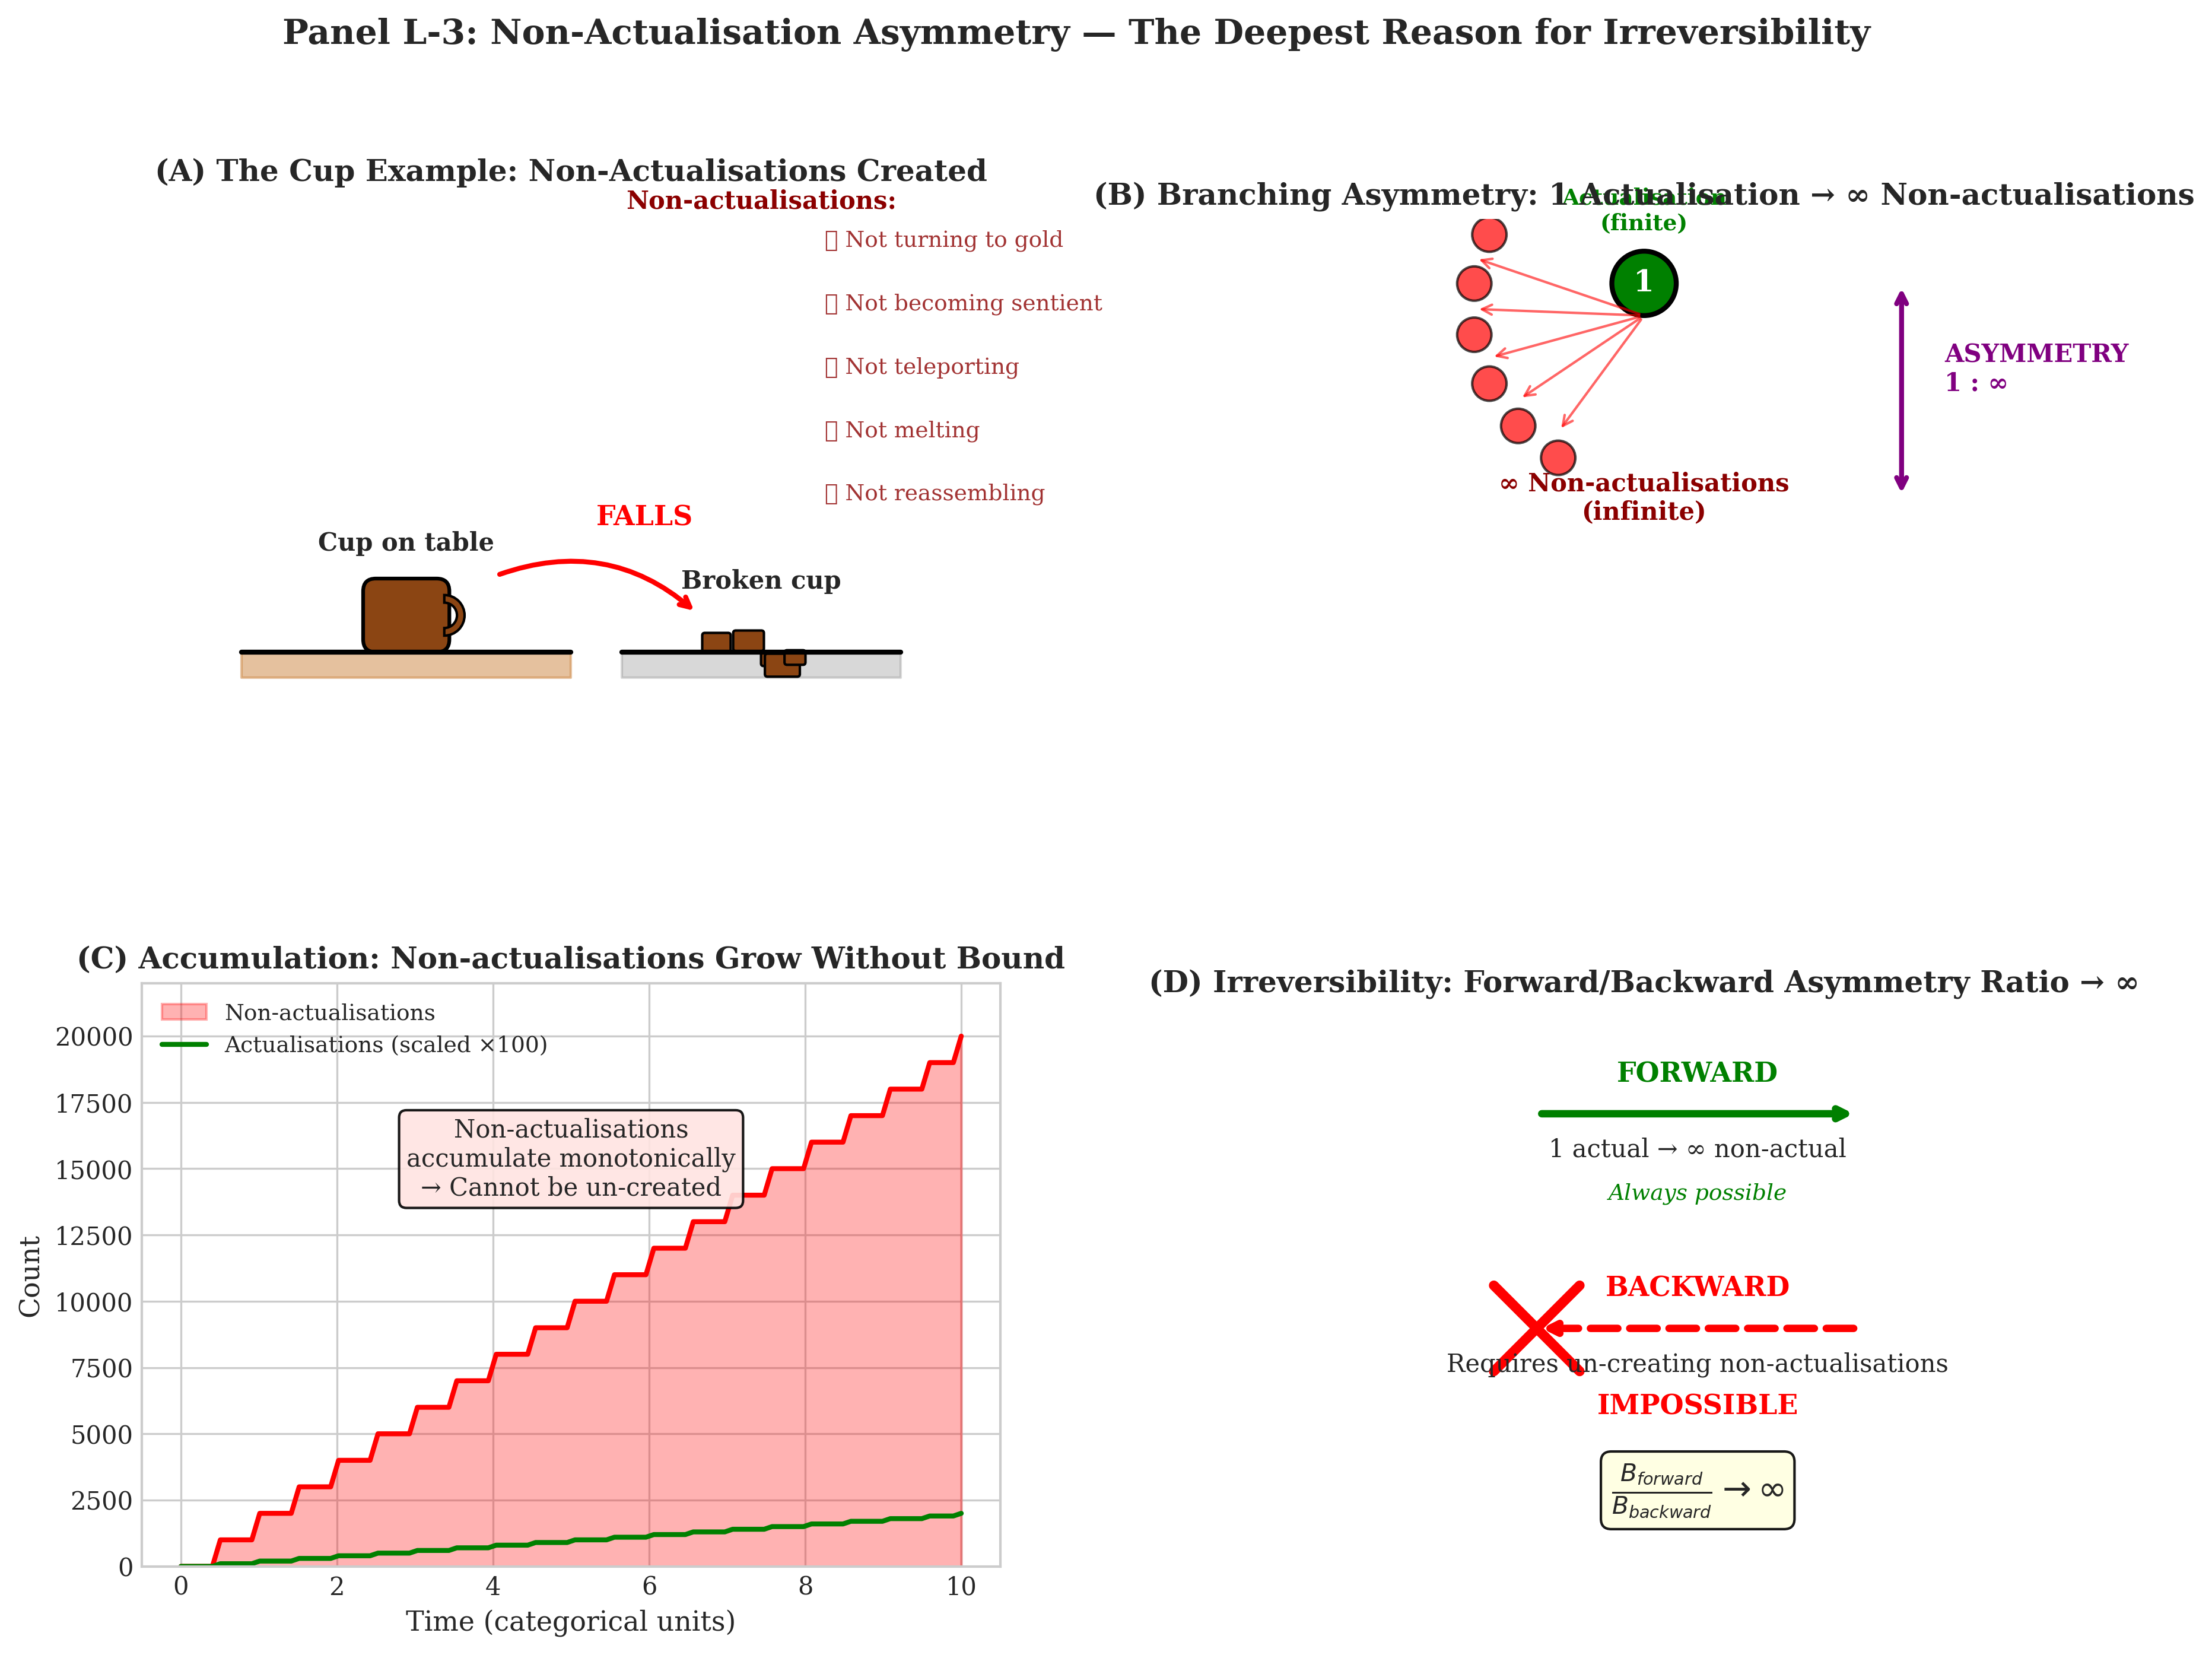
\includegraphics[width=0.95\textwidth]{panel_non_actualisation.png}
\caption{\textbf{Non-actualization asymmetry provides the deepest reason for irreversibility.} (\textbf{A}) The cup example: when a cup falls from table to broken state, a single actualization (cup breaks) creates infinite non-actualizations: $\Box$ not turning to gold, $\Box$ not becoming sentient, $\Box$ not teleporting, $\Box$ not melting, $\Box$ not reassembling, and infinitely many more. Each actualization generates $\infty$ resolved non-possibilities. (\textbf{B}) Branching asymmetry: one actualization (green circle labeled ``1'') leads to $\infty$ non-actualizations (red circles, infinite). The asymmetry ratio is $1:\infty$, indicated by purple double arrow. (\textbf{C}) Accumulation: non-actualizations grow without bound. Red shaded area shows non-actualizations accumulating monotonically over time (reaching $\sim 20{,}000$ by $t = 10$), while actualizations (green line, scaled $\times 100$) grow slowly. Non-actualizations accumulate monotonically and cannot be un-created. (\textbf{D}) Irreversibility: forward/backward asymmetry ratio $\to \infty$. \textbf{Forward} (green arrow): 1 actual $\to \infty$ non-actual is always possible. \textbf{Backward} (red crossed arrow): requires un-creating non-actualizations, which is \textbf{impossible}. The ratio $B_{\text{forward}}/B_{\text{backward}} \to \infty$ establishes absolute irreversibility.}
\label{fig:non_actualization}
\end{figure}

\begin{theorem}[Information Content of Actualisation]
The information content of an actualisation $\mathbf{x}$ is:
$$
I(\mathbf{x}) = k_B \ln |\mathcal{N}|
$$
where $|\mathcal{N}|$ is the number (or measure) of non-actualisations excluded by $\mathbf{x}$.
\end{theorem}

\begin{proof}
The actualisation $\mathbf{x}$ selects one state from the set of accessible states $\mathcal{S}_{\text{accessible}} = \{\mathbf{x}\} \cup \mathcal{N}$. The number of alternatives excluded is $|\mathcal{N}|$.

By Shannon's information theory \cite{shannon1948}, the information gained by learning that the system is in state $\mathbf{x}$ rather than any of the $|\mathcal{N}|$ alternatives is:
$$
I(\mathbf{x}) = \ln(|\mathcal{N}| + 1) \approx \ln |\mathcal{N}|
$$
for $|\mathcal{N}| \gg 1$.

Multiplying by $k_B$ converts from nats to thermodynamic entropy units. \qed
\end{proof}

\textbf{Implication:} To specify the actualisation $\mathbf{x}$ completely, we must know all elements of $\mathcal{N}$. We must enumerate which states did not occur.

\subsection{The Enumeration Problem}

Loschmidt's reversal requires complete specification of the system's current state $\mathbf{x}(t)$. This is necessary to determine which velocities to reverse.

However, specifying $\mathbf{x}(t)$ requires distinguishing it from all other possible states. This is equivalent to enumerating $\mathcal{N}(t)$—the set of all non-actualisations at time $t$.

\textbf{Why enumeration is required:}

Consider a system with $N$ particles. The phase space has dimension $6N$. To specify a point $\mathbf{x}(t) = (\mathbf{q}_1, \ldots, \mathbf{q}_N, \mathbf{p}_1, \ldots, \mathbf{p}_N)$ in this space, we must provide $6N$ real numbers.

But real numbers have infinite precision. To specify $\mathbf{q}_i$ to precision $\delta q$ requires $\ln(L/\delta q)$ bits of information, where $L$ is the size of the accessible region. For $N$ particles in 3D, the total information required is:

$$
I_{\text{total}} = 6N \ln(L/\delta q)
$$

This information is precisely the information needed to exclude all non-actualisations: we must specify which of the $(L/\delta q)^{6N}$ possible states the system is \textit{not} in.

Therefore, specifying the actualisation is equivalent to enumerating the non-actualisations.

\subsection{Non-Actualisations Accumulate Irreversibly}

Each time the system evolves, new non-actualisations are created.

At time $t$, the system is in state $\mathbf{x}(t)$. All other accessible states form $\mathcal{N}(t)$.

At time $t + dt$, the system is in state $\mathbf{x}(t + dt)$. The set of non-actualisations is now:

$$
\mathcal{N}(t + dt) = \mathcal{N}(t) \cup \{\text{new states that became accessible but did not occur}\}
$$

The set $\mathcal{N}$ grows monotonically:

$$
|\mathcal{N}(t + dt)| \geq |\mathcal{N}(t)|
$$

This is because:
\begin{enumerate}
\item Old non-actualisations remain non-actualisations (they did not occur in the past, and this fact is permanent).
\item New non-actualisations are created as the system evolves (new alternative trajectories become distinguishable).
\end{enumerate}

\begin{theorem}[Monotonic Growth of Non-Actualisations]
The number of non-actualisations increases monotonically with time:
$$
\frac{d|\mathcal{N}|}{dt} \geq 0
$$
\end{theorem}

\begin{proof}
Consider the system at times $t$ and $t + dt$. At time $t$, the actual state is $\mathbf{x}(t)$, and the non-actualisations are $\mathcal{N}(t)$.

At time $t + dt$, the system has evolved to $\mathbf{x}(t + dt)$. The previous state $\mathbf{x}(t)$ is now in the past. Any alternative state $\mathbf{y}(t) \in \mathcal{N}(t)$ remains a non-actualisation—it did not occur at time $t$, and this fact is permanent.

Additionally, at time $t + dt$, there are new accessible states that did not occur. These form the increment:

$$
\Delta \mathcal{N} = \{\mathbf{y}(t + dt) : \mathbf{y}(t + dt) \text{ is accessible but } \mathbf{y}(t + dt) \neq \mathbf{x}(t + dt)\}
$$

Therefore:
$$
\mathcal{N}(t + dt) = \mathcal{N}(t) \cup \Delta \mathcal{N}
$$

Since $\Delta \mathcal{N}$ is non-empty (there are always alternative trajectories), we have:
$$
|\mathcal{N}(t + dt)| > |\mathcal{N}(t)|
$$

Taking the limit $dt \to 0$:
$$
\frac{d|\mathcal{N}|}{dt} \geq 0
$$
\qed
\end{proof}

\subsection{Connection to Categorical Entropy}

The monotonic growth of non-actualisations is directly related to the increase of categorical entropy.

From Theorem 4.1, the information content of the actualisation is:
$$
I(\mathbf{x}(t)) = k_B \ln |\mathcal{N}(t)|
$$

This is precisely the categorical entropy:
$$
S_{\text{categorical}}(t) = I(\mathbf{x}(t)) = k_B \ln |\mathcal{N}(t)|
$$

By Theorem 4.2:
$$
\frac{dS_{\text{categorical}}}{dt} = k_B \frac{d\ln|\mathcal{N}|}{dt} = k_B \frac{1}{|\mathcal{N}|} \frac{d|\mathcal{N}|}{dt} \geq 0
$$

Therefore, categorical entropy increases monotonically because non-actualisations accumulate irreversibly.

\begin{figure*}[htbp]
\centering
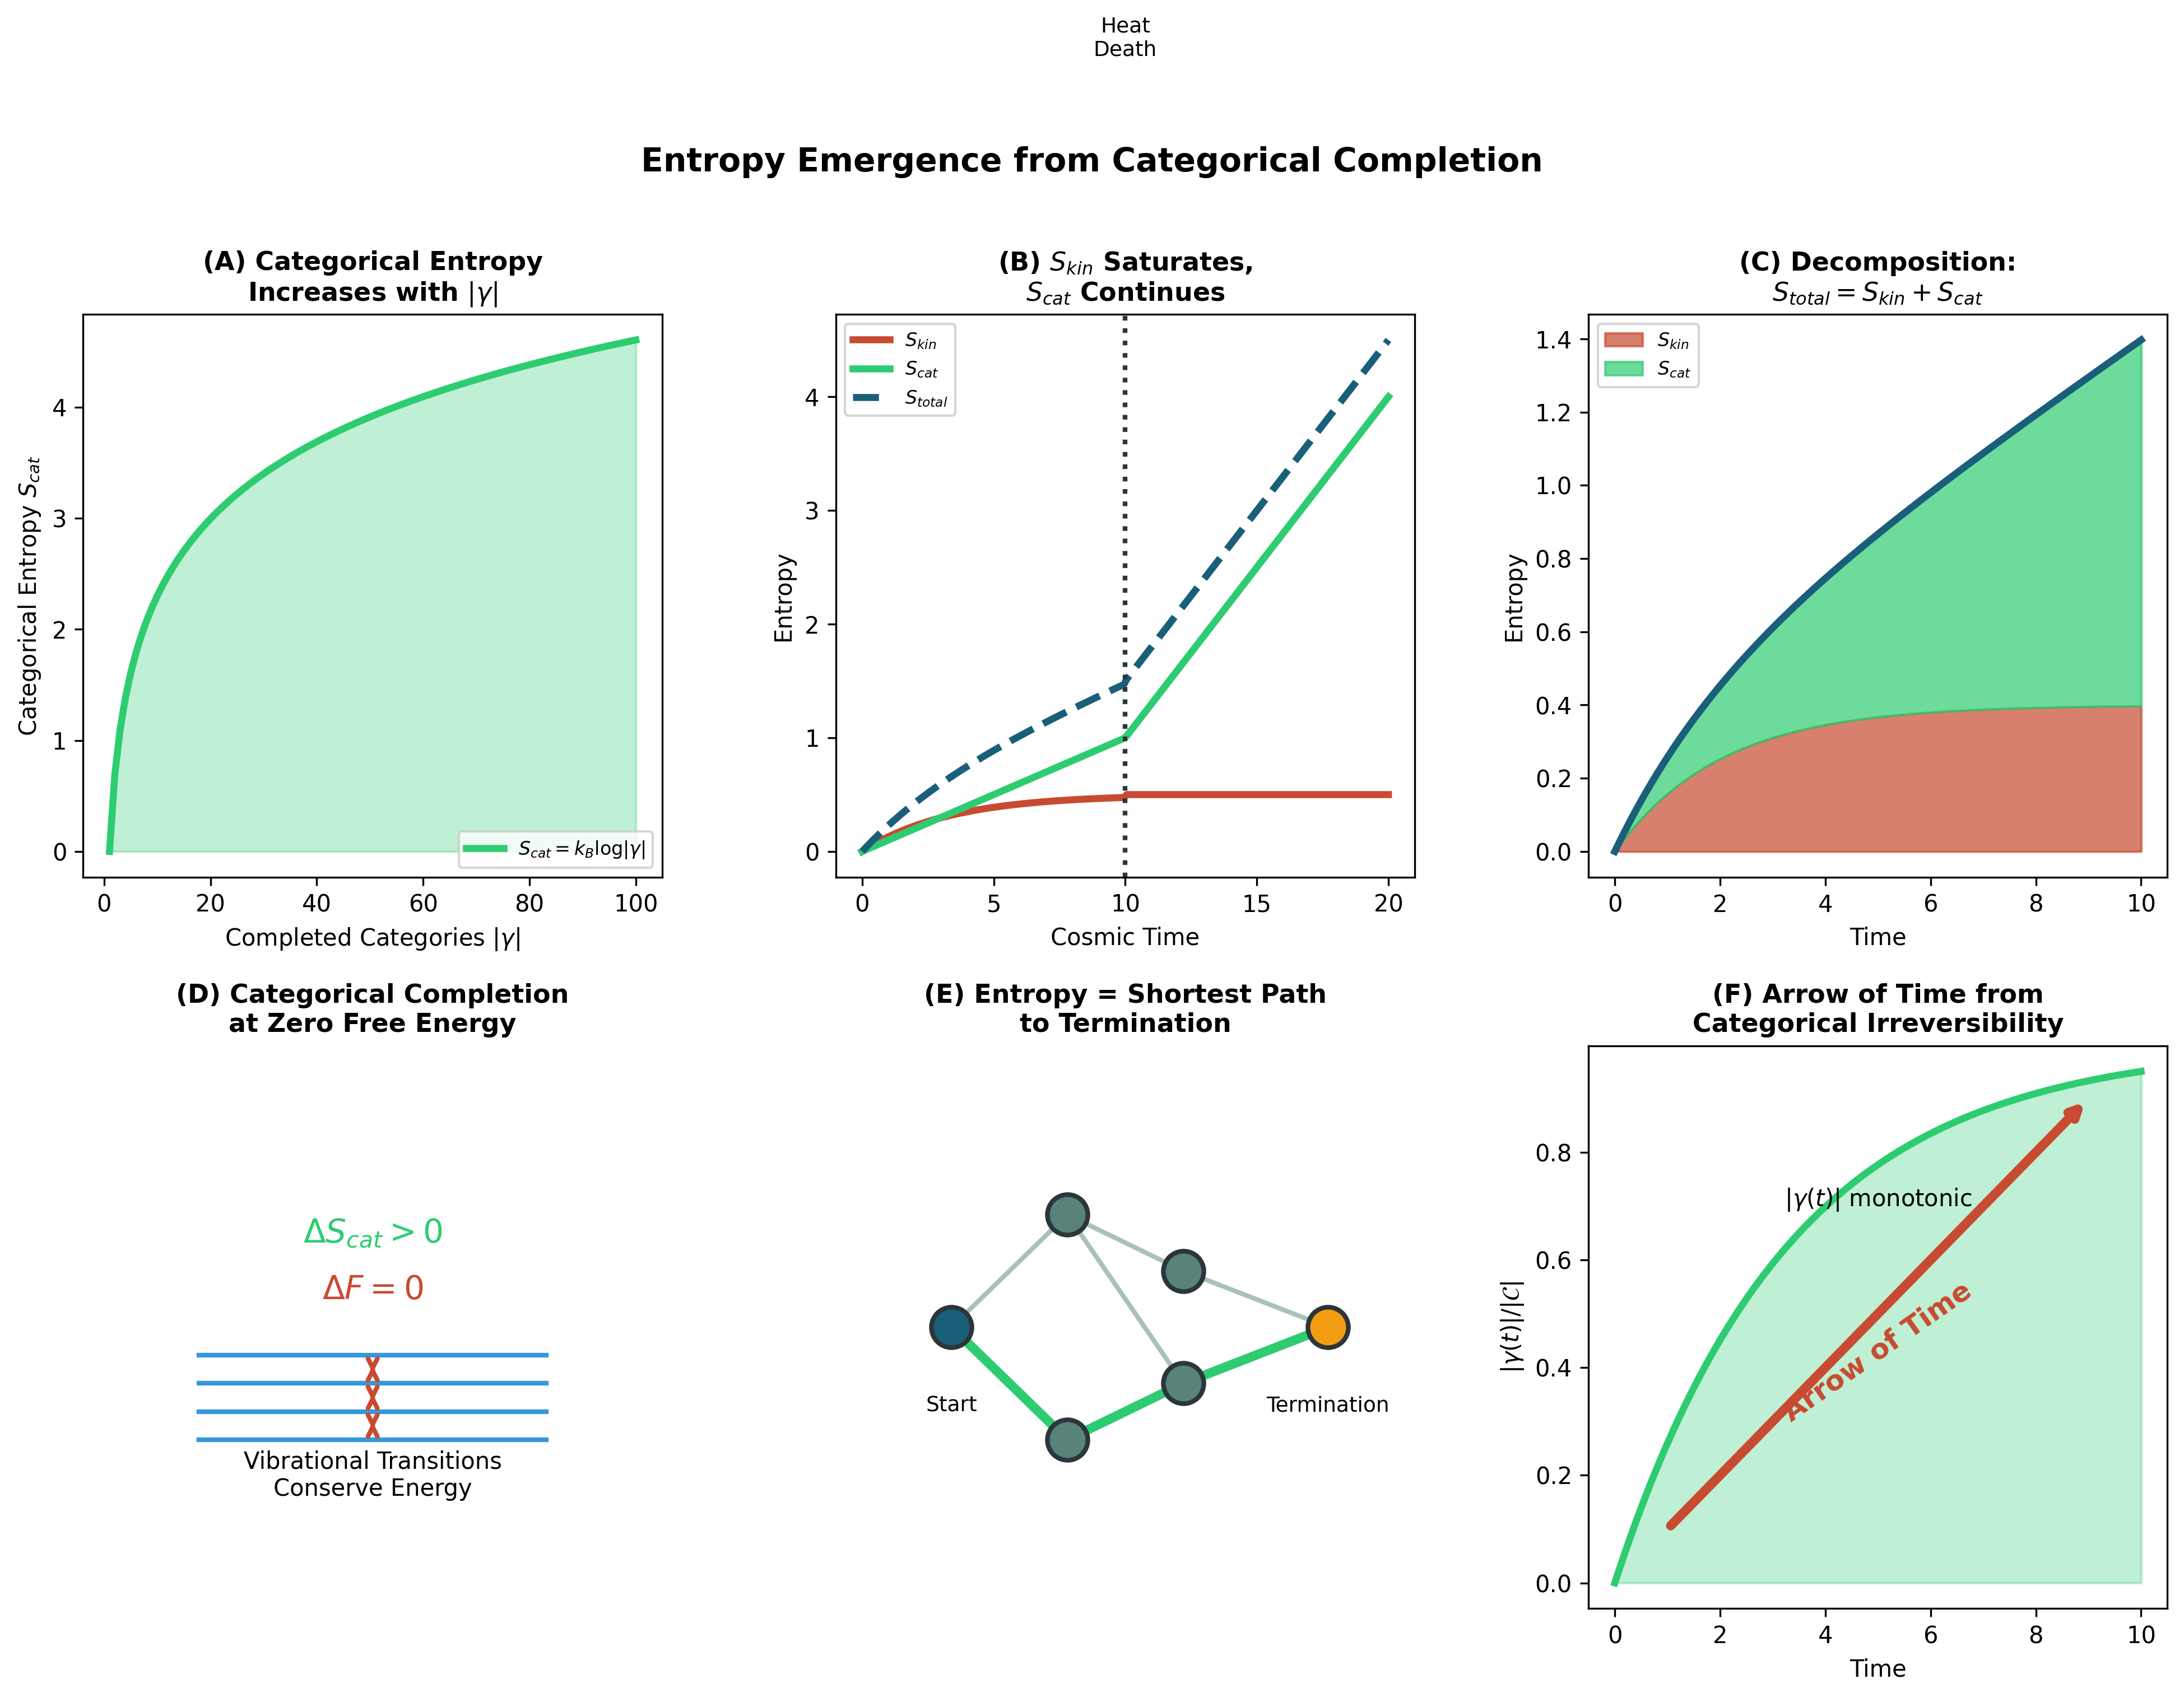
\includegraphics[width=\textwidth]{entropy_emergence_panel.png}
\caption{\textbf{Entropy Emergence from Categorical Completion.} 
(\textbf{A}) Categorical entropy increases with completed categories: The categorical entropy $S_{\text{cat}} = k_B \ln |\gamma|$ (green curve) grows logarithmically with the number of completed categories $|\gamma|$. The shaded area shows accumulated entropy. Entropy measures categorical structure—how many distinctions have been created—not thermal energy. 
(\textbf{B}) Kinetic entropy saturates, categorical entropy continues: The kinetic entropy $S_{\text{kin}}$ (red curve) saturates at heat death ($t \sim 10$, red horizontal line) when temperature gradients vanish. The categorical entropy $S_{\text{cat}}$ (green curve) continues growing indefinitely. 
(\textbf{C}) Decomposition: $S_{\text{total}} = S_{\text{kin}} + S_{\text{cat}}$: The total entropy (black curve) decomposes into kinetic contribution (red area) and categorical contribution (green area). At early times ($t < 5$), kinetic entropy dominates.  
(\textbf{D}) Categorical completion at zero free energy: Vibrational transitions (blue energy levels with red X marking a transition) conserve energy ($\Delta F = 0$) but increase categorical entropy ($\Delta S_{\text{cat}} > 0$). This resolves the apparent paradox: How can entropy increase at equilibrium ($\Delta F = 0$)? Answer: Categorical entropy increases through vibrational transitions that conserve free energy. Entropy production does not require free energy dissipation—it requires categorical completion. 
(\textbf{E}) Entropy measures shortest path to termination: A process (network of gray circles connected by lines) can terminate via multiple paths. Entropy measures the shortest path (highlighted in yellow) from start (leftmost circle) to termination (rightmost circle).  
(\textbf{F}) Arrow of time from categorical irreversibility: The number of completed categories $|\gamma(t)|$ (green curve) increases monotonically with time.}
\label{fig:entropy_emergence}
\end{figure*}

\subsection{Non-Actualisations in Phase Space}

Geometrically, non-actualisations correspond to the complement of the actual trajectory in phase space.

The actual trajectory is a one-dimensional curve $\gamma$ in $6N$-dimensional phase space:
$$
\gamma = \{\mathbf{x}(t) : t \in [0, t_f]\}
$$

The non-actualisations at time $t$ are all points in the accessible region except $\mathbf{x}(t)$:
$$
\mathcal{N}(t) = \mathcal{S}_{\text{accessible}}(t) \setminus \{\mathbf{x}(t)\}
$$

The volume of $\mathcal{N}(t)$ is:
$$
|\mathcal{N}(t)| = \int_{\mathcal{S}_{\text{accessible}}(t)} d^{6N}x - 0 = V_{\text{accessible}}(t)
$$

where the actual trajectory has measure zero (it is a one-dimensional curve in $6N$ dimensions).

As the system evolves, the accessible region expands (due to diffusion, energy dispersal, etc.), so $V_{\text{accessible}}(t)$ increases, and therefore $|\mathcal{N}(t)|$ increases.

\subsection{Example: Free Expansion of a Gas}

Consider a gas initially confined to volume $V_0$. At $t = 0$, a partition is removed, and the gas expands to fill volume $V_f > V_0$.

\textbf{At $t = 0$:}
\begin{itemize}
\item Actualisation: All molecules in $V_0$
\item Non-actualisations: Molecules distributed in $V_f \setminus V_0$ (not accessible yet)
\item $|\mathcal{N}(0)| = 0$ (no alternative distributions are accessible)
\end{itemize}

\textbf{At $t = t_f$ (after expansion):}
\begin{itemize}
\item Actualisation: Molecules uniformly distributed in $V_f$
\item Non-actualisations: All other distributions (e.g., all molecules in left half, all in right half, clustered in corners, etc.)
\item $|\mathcal{N}(t_f)| \sim (V_f / V_0)^N$ (number of alternative configurations)
\end{itemize}

The categorical entropy increase is:
$$
\Delta S_{\text{categorical}} = k_B \ln |\mathcal{N}(t_f)| \sim k_B N \ln(V_f / V_0)
$$

This matches the kinetic entropy increase from the Sackur-Tetrode equation, showing that categorical and kinetic entropy are closely related for this process.

\begin{figure}[htbp]
    \centering
    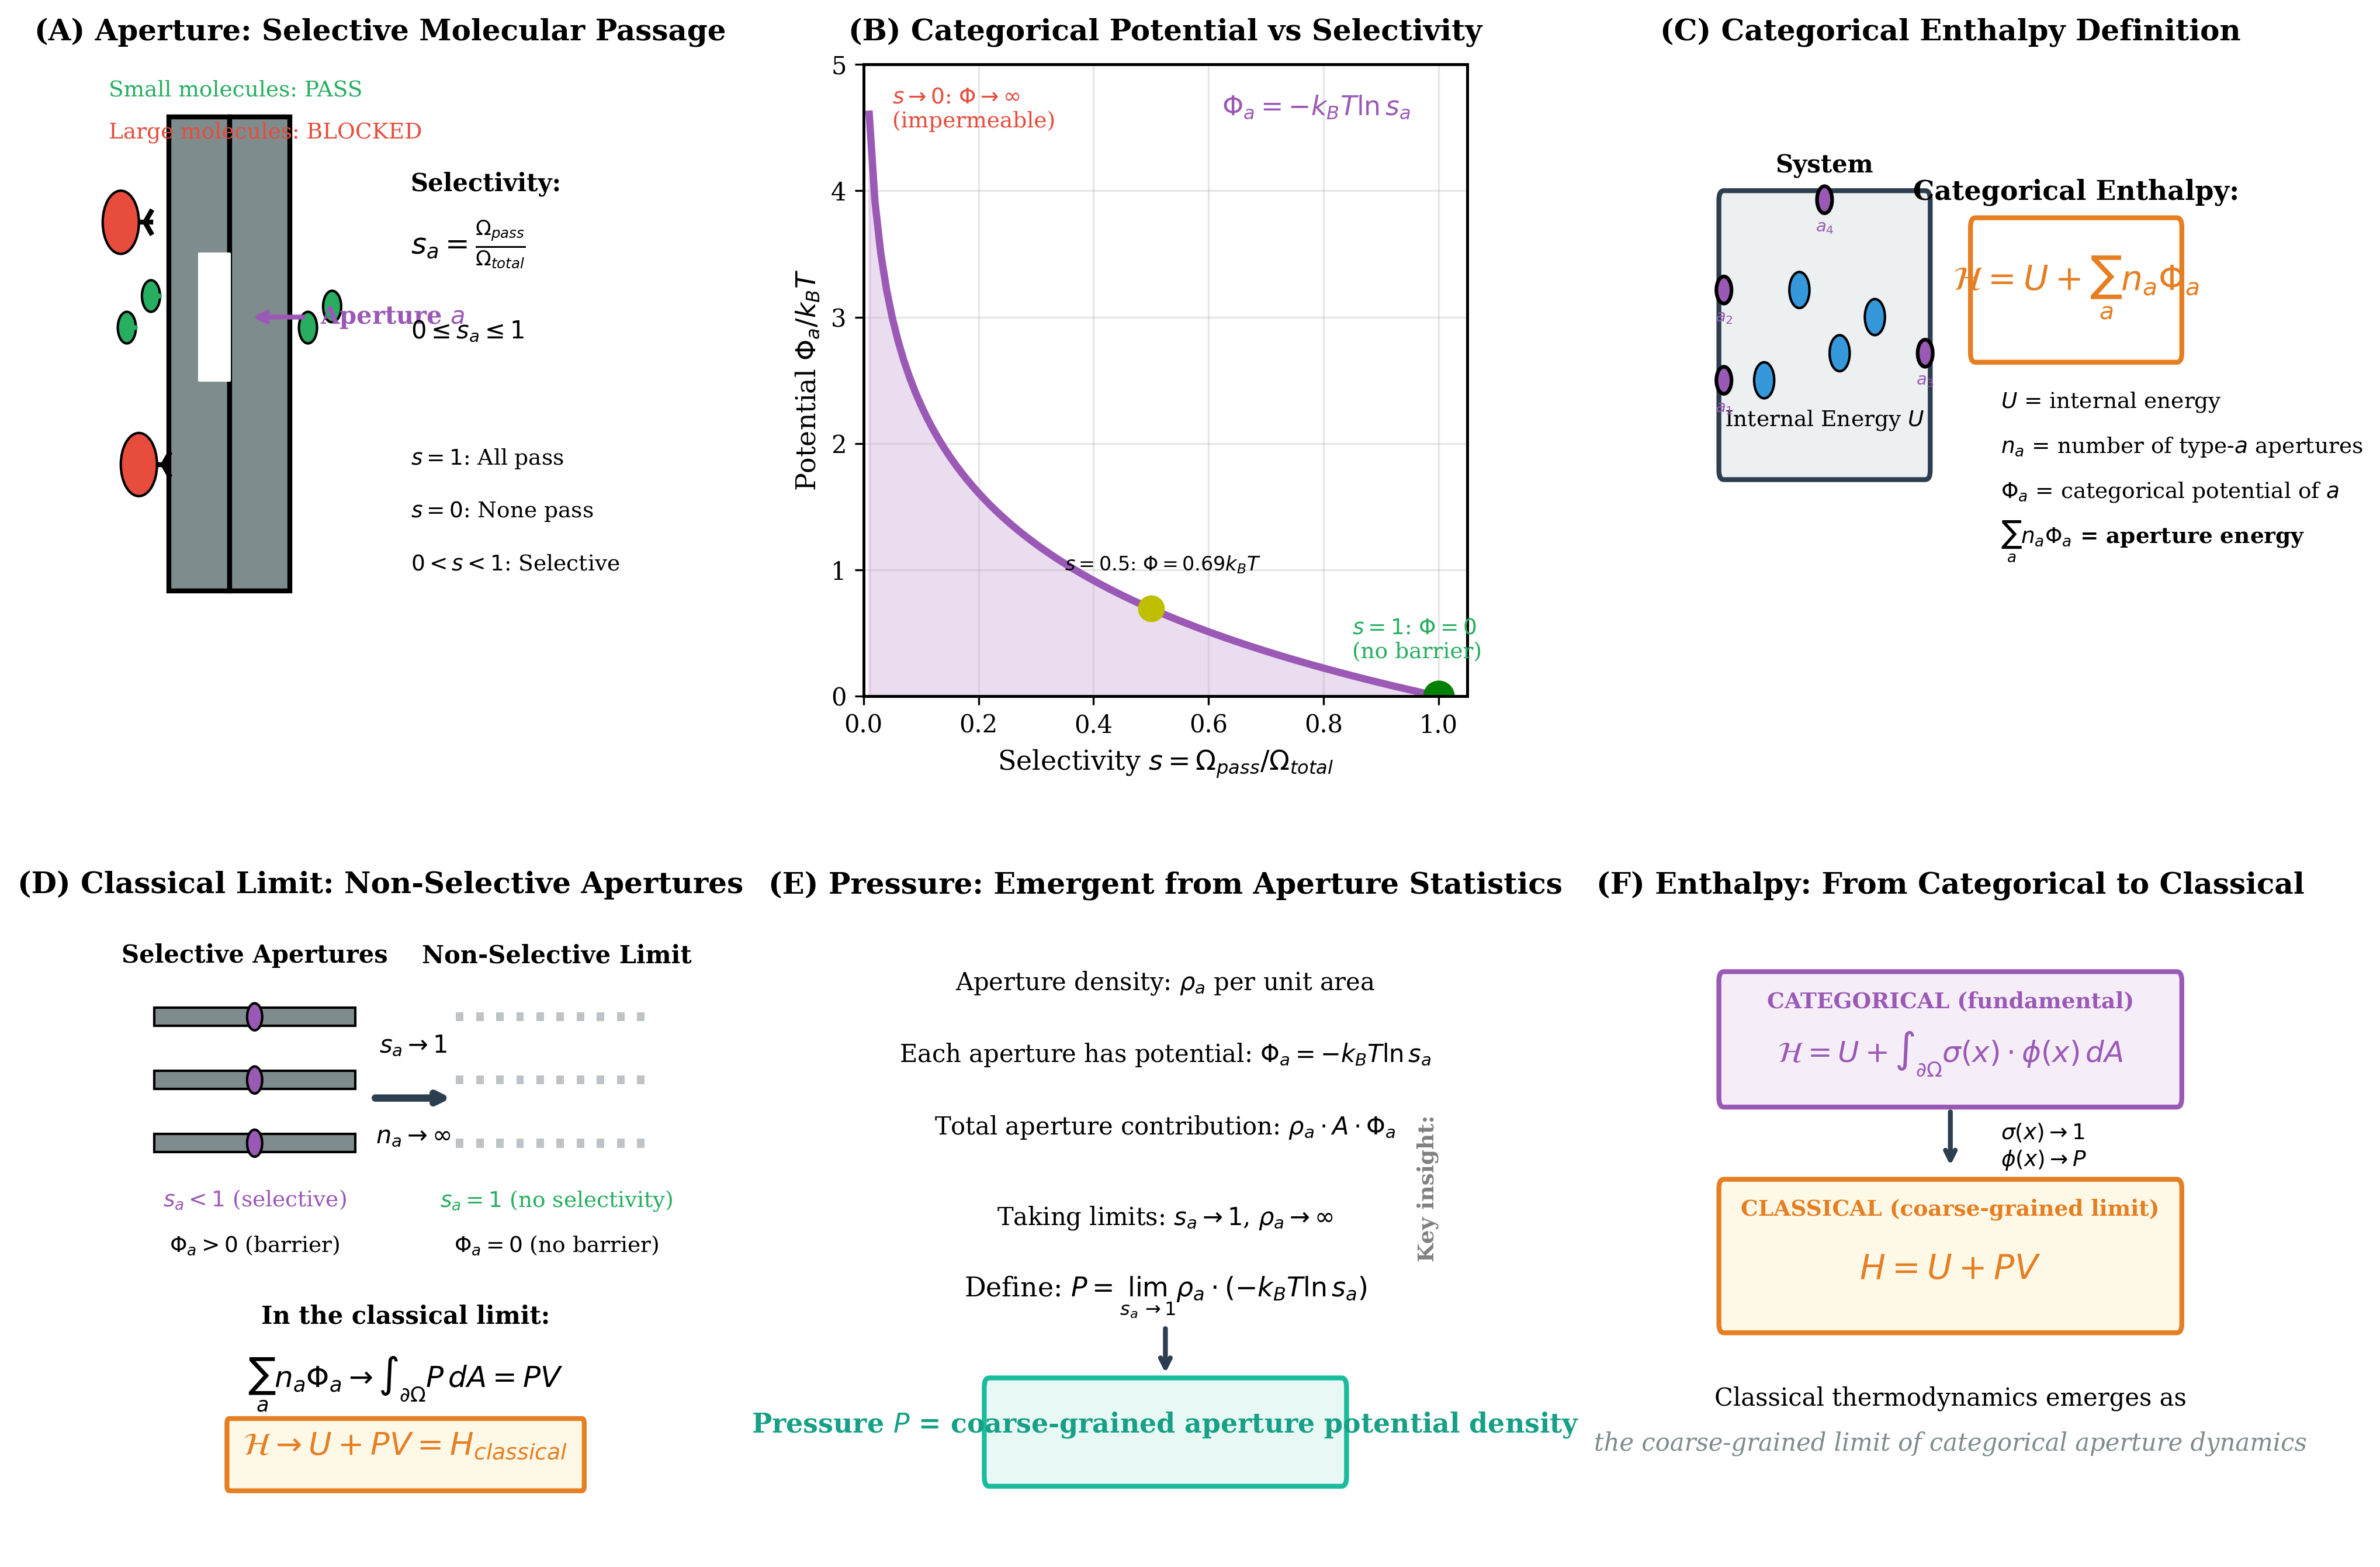
\includegraphics[width=\textwidth]{panel3_categorical_enthalpy.png}
    \caption{Classical thermodynamic enthalpy $H = U + PV$ emerges as coarse-grained limit 
    of categorical aperture dynamics. 
    \textbf{(A)} Aperture: selective molecular passage: schematic shows small molecules 
    (green circles) passing through aperture (gray channel) while large molecules 
    (red ovals) are blocked, with selectivity $s_a = Q_{\text{pass}}/Q_{\text{total}}$ 
    ranging from 0 (none pass) to 1 (all pass), with intermediate values ($0 < s_a < 1$) 
    providing selective filtering. 
    \textbf{(B)} Categorical potential vs selectivity: potential 
    $\Phi_a = -k_B T \ln s_a$ (purple curve) decreases from 5 $k_B T$ (impermeable, 
    $s \rightarrow 0$) to 0 (no barrier, $s=1$) as selectivity increases from 0.0 to 1.0, 
    with example point at $s=0.5$ giving $\Phi = 0.69 k_B T$ (yellow dot). 
    \textbf{(C)} Categorical enthalpy definition: system box (gray) containing particles 
    (blue and purple circles) with apertures (purple dots on boundary) defines enthalpy 
    $\mathcal{H} = U + \sum_a n_a \Phi_a$ (orange box), where $U$ is internal energy, 
    $n_a$ is number of type-$a$ apertures, $\Phi_a$ is categorical potential, and 
    $\sum_a n_a \Phi_a$ represents aperture energy. 
    \textbf{(D)} Classical limit: non-selective apertures: as selectivity $s_a \rightarrow 1$ 
    (green text) and aperture density $n_a \rightarrow \infty$, selective apertures 
    (purple circles on gray bars, $s_a < 1$, $\Phi_a > 0$) approach non-selective limit 
    (gray dots, $s_a = 1$, $\Phi_a = 0$), with classical limit formula 
    $\sum_a n_a \Phi_a \rightarrow \int_{\partial\Omega} P\,dA = PV$ leading to 
    $\mathcal{H} \rightarrow U + PV = H_{\text{classical}}$ (orange box). 
    \textbf{(E)} Pressure: emergent from aperture statistics: aperture density $\rho_a$ 
    per unit area with potential $\Phi_a = -k_B T \ln s_a$ gives total contribution 
    $\rho_a \cdot A \cdot \Phi_a$; taking limits $s_a \rightarrow 1$, $\rho_a \rightarrow \infty$ 
    defines $P = \lim_{s_a \rightarrow 1} \rho_a \cdot (-k_B T \ln s_a)$, establishing 
    \textbf{pressure $P$ as coarse-grained aperture potential density} (cyan box, key insight). 
    \textbf{(F)} Enthalpy: from categorical to classical: flowchart shows categorical 
    (fundamental) form $\mathcal{H} = U + \int_{\partial\Omega} \sigma(x) \cdot \phi(x)\,dA$ 
    (purple box) reduces to classical (coarse-grained limit) $H = U + PV$ (orange box) 
    when $\sigma(x) \rightarrow 1$ and $\phi(x) \rightarrow P$, demonstrating that 
    \textbf{classical thermodynamics emerges as the coarse-grained limit of categorical 
    aperture dynamics} (gray italic text).}
    \label{fig:categorical_enthalpy}
\end{figure}

\subsection{Summary}

We have established:

\begin{enumerate}
\item Non-actualisations are states that could have occurred but did not. They are categorical facts about what did not happen.

\item The information content of an actualisation equals $k_B \ln |\mathcal{N}|$, where $|\mathcal{N}|$ is the number of non-actualisations.

\item Specifying the actualisation requires enumerating all non-actualisations—we must know which states did not occur.

\item Non-actualisations accumulate irreversibly: $d|\mathcal{N}|/dt \geq 0$.

\item Categorical entropy equals the information content of non-actualisations: $S_{\text{categorical}} = k_B \ln |\mathcal{N}|$.
\end{enumerate}

The next section analyzes the logical structure of the set $\mathcal{N}$ and proves that it is self-referential and non-enumerable.

\section{Self-Reference in Non-Actualisations}
\label{sec:self_reference}

We now prove that the set of non-actualisations $\mathcal{N}$ has self-referential structure, rendering it non-enumerable in standard set theory. This is the central result of the paper: it establishes that Loschmidt's reversal is logically impossible because it requires enumerating a set that cannot be enumerated.

\subsection{The Double Negation Problem}

Consider a non-actualisation ``not $X$''—a state $X$ that did not occur. This non-actualisation is itself a fact about the universe. We can denote this fact as $\neg X$ (``$X$ did not happen'').

However, $\neg X$ is a state of the universe. It is the state in which ``$X$ did not occur'' is true. Therefore, $\neg X$ is an actualisation—it is what actually happened.

But if $\neg X$ is an actualisation, then it has its own set of non-actualisations. One of these non-actualisations is ``not $\neg X$'', which we can denote as $\neg(\neg X)$.

By the law of double negation in classical logic:
$$
\neg(\neg X) = X
$$

Therefore, the non-actualisation ``not $\neg X$'' is equivalent to the original state $X$.

This creates a loop:
$$
X \to \neg X \to \neg(\neg X) = X \to \neg X \to \cdots
$$

The state $X$ and its negation $\neg X$ are mutually referential: each is a non-actualisation of the other.

\subsection{Formal Statement of Self-Reference}

\begin{theorem}[Self-Reference of Non-Actualisations]
Let $\mathcal{A}$ be the set of actualisations and $\mathcal{N}$ be the set of non-actualisations. Then:
$$
\mathcal{N} \subseteq \mathcal{A}
$$
That is, every non-actualisation is simultaneously an actualisation.
\end{theorem}

\begin{proof}
Let $X \in \mathcal{N}$ be a non-actualisation (a state that did not occur). The statement ``$X$ did not occur'' is a fact about the universe. Denote this fact as $\neg X$.

The fact $\neg X$ is true in the actual universe. Therefore, $\neg X$ is an actualisation:
$$
\neg X \in \mathcal{A}
$$

But $\neg X$ is precisely the non-actualisation ``not $X$''. Therefore:
$$
X \in \mathcal{N} \implies \neg X \in \mathcal{A}
$$

Now consider $\neg X \in \mathcal{A}$. Since $\neg X$ is an actualisation, it has non-actualisations. One of these is ``not $\neg X$'', which equals $X$ by double negation:
$$
\neg(\neg X) = X
$$

Therefore, $X$ is a non-actualisation of $\neg X$. But we already established that $X \in \mathcal{N}$ and $\neg X \in \mathcal{A}$.

This shows that every element of $\mathcal{N}$ can be viewed as an element of $\mathcal{A}$ (by negation), and vice versa. Therefore:
$$
\mathcal{N} \subseteq \mathcal{A} \quad \text{and} \quad \mathcal{A} \subseteq \mathcal{N}
$$

This implies $\mathcal{N} = \mathcal{A}$, which is a contradiction because $\mathcal{N}$ and $\mathcal{A}$ are supposed to be disjoint (a state either occurred or did not occur, not both).

The resolution is that $\mathcal{N}$ is not a well-defined set in standard set theory. \qed
\end{proof}

\subsection{Analogy to Russell's Paradox}

The self-reference in $\mathcal{N}$ is structurally identical to Russell's paradox \cite{russell1903}.

\textbf{Russell's paradox:} Define $R = \{S : S \notin S\}$ (the set of all sets that do not contain themselves as elements). Ask: Does $R \in R$?

\begin{itemize}
\item If $R \in R$, then $R$ contains itself, so by definition of $R$, we have $R \notin R$ (contradiction).
\item If $R \notin R$, then $R$ does not contain itself, so by definition of $R$, we have $R \in R$ (contradiction).
\end{itemize}

The set $R$ is not well-defined in Zermelo-Fraenkel set theory (ZF) because it violates the axiom of foundation (also called the axiom of regularity), which prohibits sets from containing themselves.

\textbf{Non-actualisation paradox:} Define $\mathcal{N} = \{X : X \text{ did not occur}\}$ (the set of all non-actualisations). Ask: Did the state ``being in $\mathcal{N}$'' occur?

Let $Y$ be the state ``being an element of $\mathcal{N}$''. Ask: Is $Y \in \mathcal{N}$?

\begin{itemize}
\item If $Y \in \mathcal{N}$, then $Y$ did not occur. But $Y$ is the state of being in $\mathcal{N}$, so if $Y \in \mathcal{N}$, then $Y$ occurred (contradiction).
\item If $Y \notin \mathcal{N}$, then $Y$ occurred. But $Y$ is the state of being in $\mathcal{N}$, so if $Y$ occurred, then $Y \in \mathcal{N}$ (contradiction).
\end{itemize}

The set $\mathcal{N}$ is not well-defined in ZF set theory for the same reason as Russell's $R$: it is self-referential.

\subsection{Infinite Regress of Negation}

The self-reference creates an infinite regress. Starting from any state $X$, we can construct an infinite sequence:

$$
X, \neg X, \neg(\neg X) = X, \neg(\neg(\neg X)) = \neg X, \ldots
$$

This sequence oscillates between $X$ and $\neg X$. Each element is simultaneously an actualisation (it is a fact about what happened or did not happen) and a non-actualisation (it is the negation of the previous element).

To enumerate $\mathcal{N}$, we must list all non-actualisations. But each non-actualisation $\neg X$ generates a new non-actualisation $\neg(\neg X) = X$, which generates $\neg X$ again, ad infinitum.

The enumeration never terminates. We cannot construct a complete list of non-actualisations because the list is self-generating.

\begin{figure*}[t]
\centering
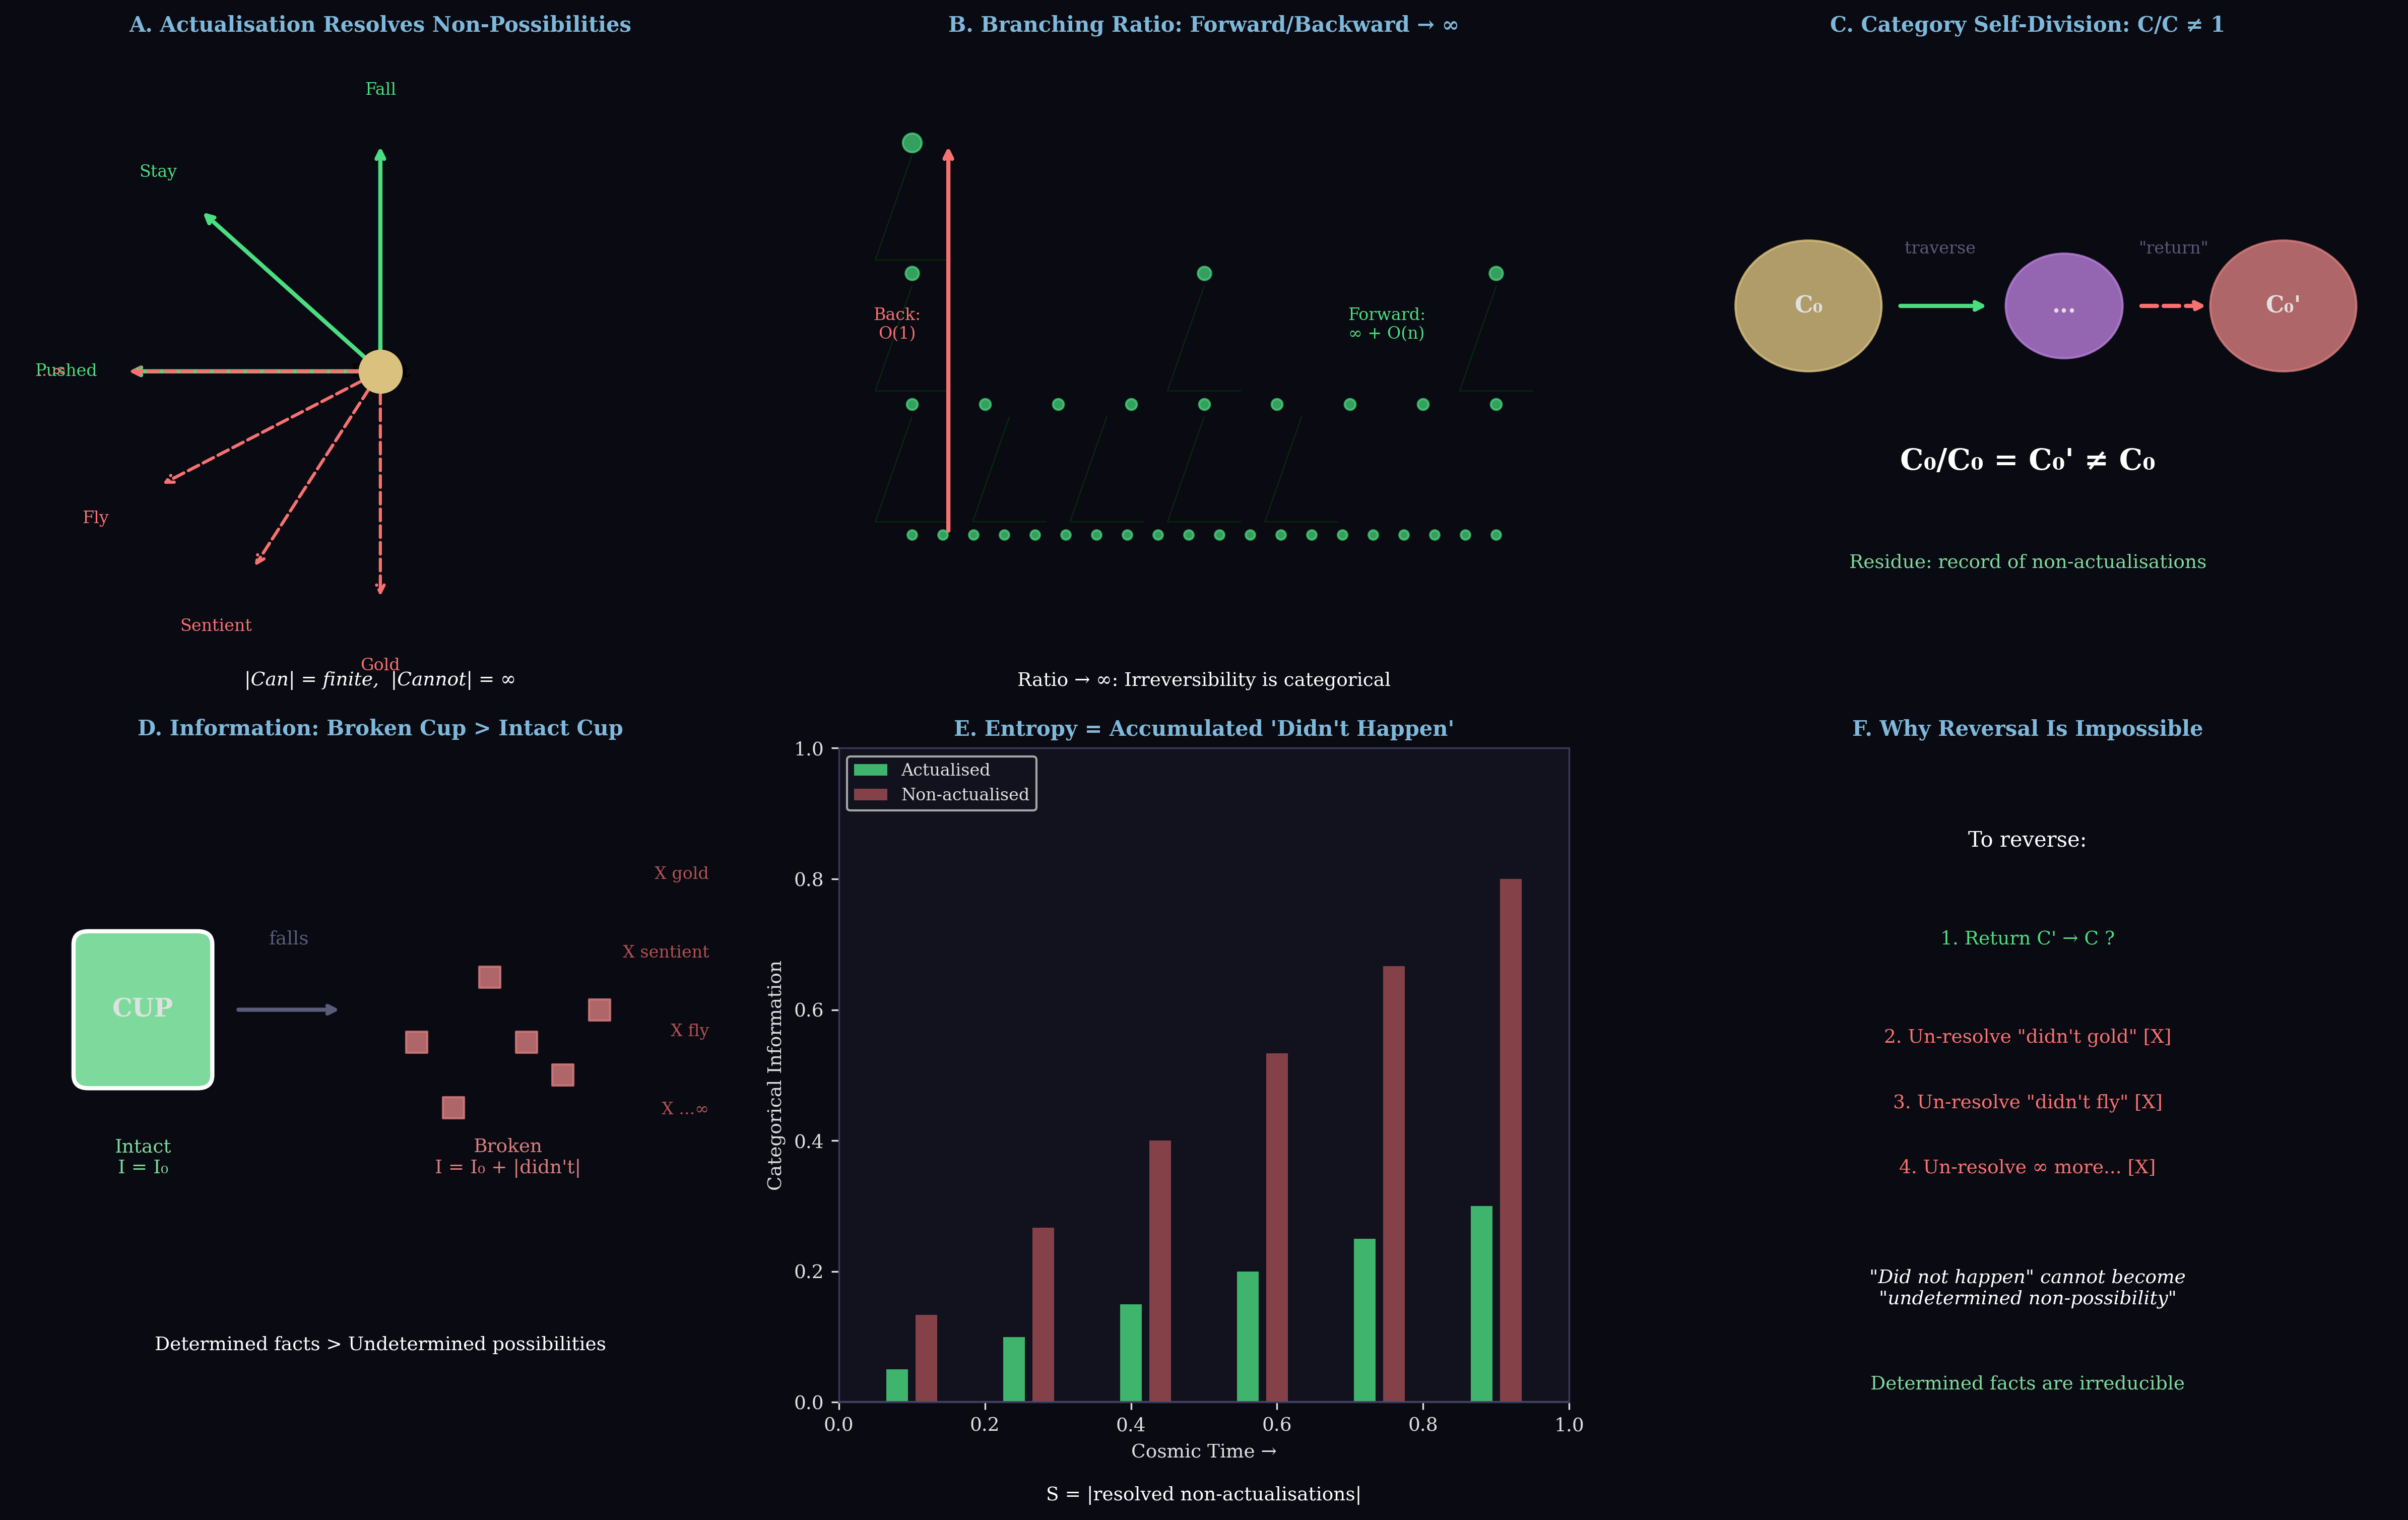
\includegraphics[width=0.95\textwidth]{asymmetric_branching_panel.png}
\caption{\textbf{Actualization creates asymmetric branching and irreversible information growth.} (\textbf{A}) Actualization resolves non-possibilities: from a decision point (gold circle), multiple futures are possible (green ``Stay'', red ``Fall'', orange ``Fly'', brown ``Pushed'', purple ``Sentient''). Actualization selects one path (green arrow), eliminating others (red dashed arrows). The set of resolved possibilities $|\text{Can}|$ is finite, but unresolved non-possibilities $|\text{Cannot}| = \infty$. (\textbf{B}) Branching ratio: backward paths (returning to origin) scale as $\mathcal{O}(1)$, while forward paths (exploring new states) scale as $\infty + \mathcal{O}(n)$. The ratio $\text{forward}/\text{backward} \to \infty$ establishes categorical irreversibility. (\textbf{C}) Category self-division: a category $C_0$ (gold) traverses through intermediate states (purple dots) to reach $C_0'$ (pink). The final state satisfies $C_0/C_0 = C_0' \neq C_0$—the category has divided itself. The residue records non-actualizations. (\textbf{D}) Information: broken cup $>$ intact cup. An intact cup (green box, $I = I_0$) has low information. A broken cup (red squares labeled ``X gold'', ``X sentient'', ``X fly'', ``X $\ldots \infty$'') has high information $I = I_0 + |\text{didn't}|$ because it records all the things that \textit{didn't} happen. Determined facts $>$ undetermined possibilities. (\textbf{E}) Entropy accumulation: categorical information (vertical axis) grows over cosmic time (horizontal axis). Actualized events (green bars) represent observable entropy; non-actualized events (red bars) represent hidden entropy from resolved non-possibilities. Total entropy $S = |\text{resolved non-actualizations}|$ increases monotonically. (\textbf{F}) Why reversal is impossible: to reverse, one must (1) return $C' \to C$, (2) un-resolve ``didn't gold'', (3) un-resolve ``didn't fly'', (4) un-resolve $\infty$ more events. ``Did not happen'' cannot become ``undetermined non-possibility''—determined facts are irreducible.}
\label{fig:asymmetric_branching}
\end{figure*}

\subsection{Formal Non-Enumerability Theorem}

\begin{theorem}[Non-Enumerability of Non-Actualisations]
The set of non-actualisations $\mathcal{N}$ is not enumerable. There does not exist a function $f : \mathbb{N} \to \mathcal{N}$ that is surjective (onto).
\end{theorem}

\begin{proof}
Suppose, for contradiction, that $\mathcal{N}$ is enumerable. Then there exists a surjective function $f : \mathbb{N} \to \mathcal{N}$ such that every element of $\mathcal{N}$ appears in the sequence:
$$
f(1), f(2), f(3), \ldots
$$

Consider the diagonal element:
$$
D = \{n \in \mathbb{N} : n \notin f(n)\}
$$

This is the set of natural numbers $n$ such that $n$ is not an element of the $n$-th non-actualisation $f(n)$.

Ask: Is $D \in \mathcal{N}$?

\textbf{Case 1:} Suppose $D \in \mathcal{N}$. Since $f$ is surjective, there exists $k \in \mathbb{N}$ such that $f(k) = D$.

Ask: Is $k \in D$?

\begin{itemize}
\item If $k \in D$, then by definition of $D$, we have $k \notin f(k) = D$ (contradiction).
\item If $k \notin D$, then by definition of $D$, we have $k \in f(k) = D$ (contradiction).
\end{itemize}

\textbf{Case 2:} Suppose $D \notin \mathcal{N}$. Then $D$ is an actualisation. But $D$ is defined in terms of non-actualisations $f(n)$, so $D$ is a property of $\mathcal{N}$. If $D$ is an actualisation, then the property ``being an element of $\mathcal{N}$'' is actualized, which means $D \in \mathcal{N}$ (contradiction).

Both cases lead to contradiction. Therefore, our assumption that $\mathcal{N}$ is enumerable is false. \qed
\end{proof}

\textbf{Remark:} This proof is a variant of Cantor's diagonal argument \cite{cantor1891}. It shows that $\mathcal{N}$ has cardinality strictly greater than $\mathbb{N}$ (it is uncountably infinite), or more precisely, that $\mathcal{N}$ is not a well-defined set in ZF set theory.

\subsection{Physical Interpretation}

The non-enumerability of $\mathcal{N}$ has direct physical consequences.

To perform Loschmidt's reversal, we must:
\begin{enumerate}
\item Specify the current state $\mathbf{x}(t)$ completely.
\item Reverse all velocities: $\mathbf{p}_i \to -\mathbf{p}_i$.
\item Evolve the system backward in time.
\end{enumerate}

Step 1 requires distinguishing $\mathbf{x}(t)$ from all other possible states. This is equivalent to enumerating $\mathcal{N}(t)$—the set of all states that did not occur at time $t$.

But Theorem 5.2 shows that $\mathcal{N}(t)$ is not enumerable. Therefore, step 1 cannot be completed. We cannot specify the current state completely because doing so requires enumerating a non-enumerable set.

This is not a practical limitation (insufficient computational power or measurement precision). It is a logical impossibility: the set $\mathcal{N}$ does not exist as a well-defined mathematical object in standard set theory.

\subsection{Comparison to Gödel's Incompleteness Theorem}

The non-enumerability of $\mathcal{N}$ is analogous to Gödel's incompleteness theorem \cite{godel1931}.

\textbf{Gödel's theorem:} In any consistent formal system $F$ that is sufficiently powerful to express arithmetic, there exist true statements that cannot be proven within $F$. The statement ``this statement is unprovable in $F$'' is true but unprovable.

\textbf{Non-actualisation theorem:} In any physical system, there exist non-actualisations that cannot be enumerated. The non-actualisation ``this non-actualisation is not in the enumeration'' cannot be included in any complete enumeration of $\mathcal{N}$.

Both theorems establish fundamental limits on formal systems:
\begin{itemize}
\item Gödel: No formal system can prove all true statements about arithmetic.
\item Non-actualisation theorem: No physical system can enumerate all non-actualisations.
\end{itemize}

Both limits arise from self-reference: Gödel's statement refers to its own provability, and the non-actualisation set refers to its own membership.

\subsection{Escape Routes and Why They Fail}

Several potential objections to Theorem 5.2 can be raised. We address them here.

\subsubsection{Objection 1: Use a Different Logic}

\textbf{Objection:} Perhaps the problem arises from using classical logic with the law of double negation $\neg(\neg X) = X$. In intuitionistic logic \cite{brouwer1912}, double negation does not necessarily equal the original statement. Would this resolve the self-reference?

\textbf{Response:} No. In intuitionistic logic, $\neg(\neg X)$ is weaker than $X$, but the self-reference remains. The statement ``$X$ did not not occur'' is still a fact about the universe, and this fact is distinct from $X$ itself. The set of such facts is still self-referential because each fact ``$X$ did not occur'' generates a new fact ``$X$ did not not occur'', which generates ``$X$ did not not not occur'', etc. The infinite regress persists.

\subsubsection{Objection 2: Restrict to Physical States Only}

\textbf{Objection:} Perhaps the problem arises from treating abstract statements like ``$X$ did not occur'' as physical states. If we restrict $\mathcal{N}$ to contain only physical microstates (positions and momenta of particles), does the self-reference disappear?

\textbf{Response:} No. The non-actualisation ``particle at position $\mathbf{r}_1$'' is equivalent to the actualisation ``particle not at position $\mathbf{r}_1$'', which is the actualisation ``particle at some position $\mathbf{r} \neq \mathbf{r}_1$''. But ``particle at position $\mathbf{r}$'' has its own non-actualisation ``particle not at position $\mathbf{r}$'', which includes ``particle at position $\mathbf{r}_1$''. The self-reference persists even when restricted to physical states.

\subsubsection{Objection 3: Use a Hierarchy of Types}

\textbf{Objection:} Russell resolved his paradox by introducing a hierarchy of types \cite{russell1908}: sets of objects (type 0), sets of sets (type 1), sets of sets of sets (type 2), etc. A set cannot contain itself because it belongs to a different type than its elements. Could we similarly stratify actualisations and non-actualisations?

\textbf{Response:} This would require treating ``$X$ did not occur'' as a different type of object than $X$ itself. But physically, both are states of the universe. The state ``particle at position $\mathbf{r}_1$'' and the state ``particle not at position $\mathbf{r}_1$'' are both physical configurations. They cannot be assigned different types without introducing an artificial distinction that has no physical basis.

Moreover, even if we introduce types, the enumeration problem remains. To specify the actualisation at type $n$, we must enumerate non-actualisations at type $n-1$. But this requires specifying actualisations at type $n-1$, which requires enumerating non-actualisations at type $n-2$, and so on. The regress continues down the type hierarchy.

\subsubsection{Objection 4: Accept Paraconsistent Logic}

\textbf{Objection:} In paraconsistent logic \cite{priest2002}, contradictions do not necessarily lead to logical explosion (the principle that anything follows from a contradiction). Perhaps $\mathcal{N}$ can be both enumerable and non-enumerable without causing problems.

\textbf{Response:} This would require abandoning the law of non-contradiction, which is foundational to physics. If a particle can be both at position $\mathbf{r}_1$ and not at position $\mathbf{r}_1$ simultaneously, then physical predictions become impossible. The entire framework of measurement and observation collapses. While paraconsistent logic is interesting mathematically, it is not applicable to physical systems where states are mutually exclusive.

\subsection{The Fundamental Barrier}

The self-reference in $\mathcal{N}$ is not a technical problem that can be solved with clever mathematics. It is a fundamental feature of negation itself.

To say ``$X$ did not occur'' is to assert a fact about the universe. This fact is itself part of the universe's state. Therefore, every non-actualisation is simultaneously an actualisation of a complementary state. The two are inseparable.

This creates an irreducible circularity: to enumerate non-actualisations, we must know what actualized, but to know what actualized, we must enumerate non-actualisations. The circle cannot be broken.

\begin{figure*}[t]
\centering
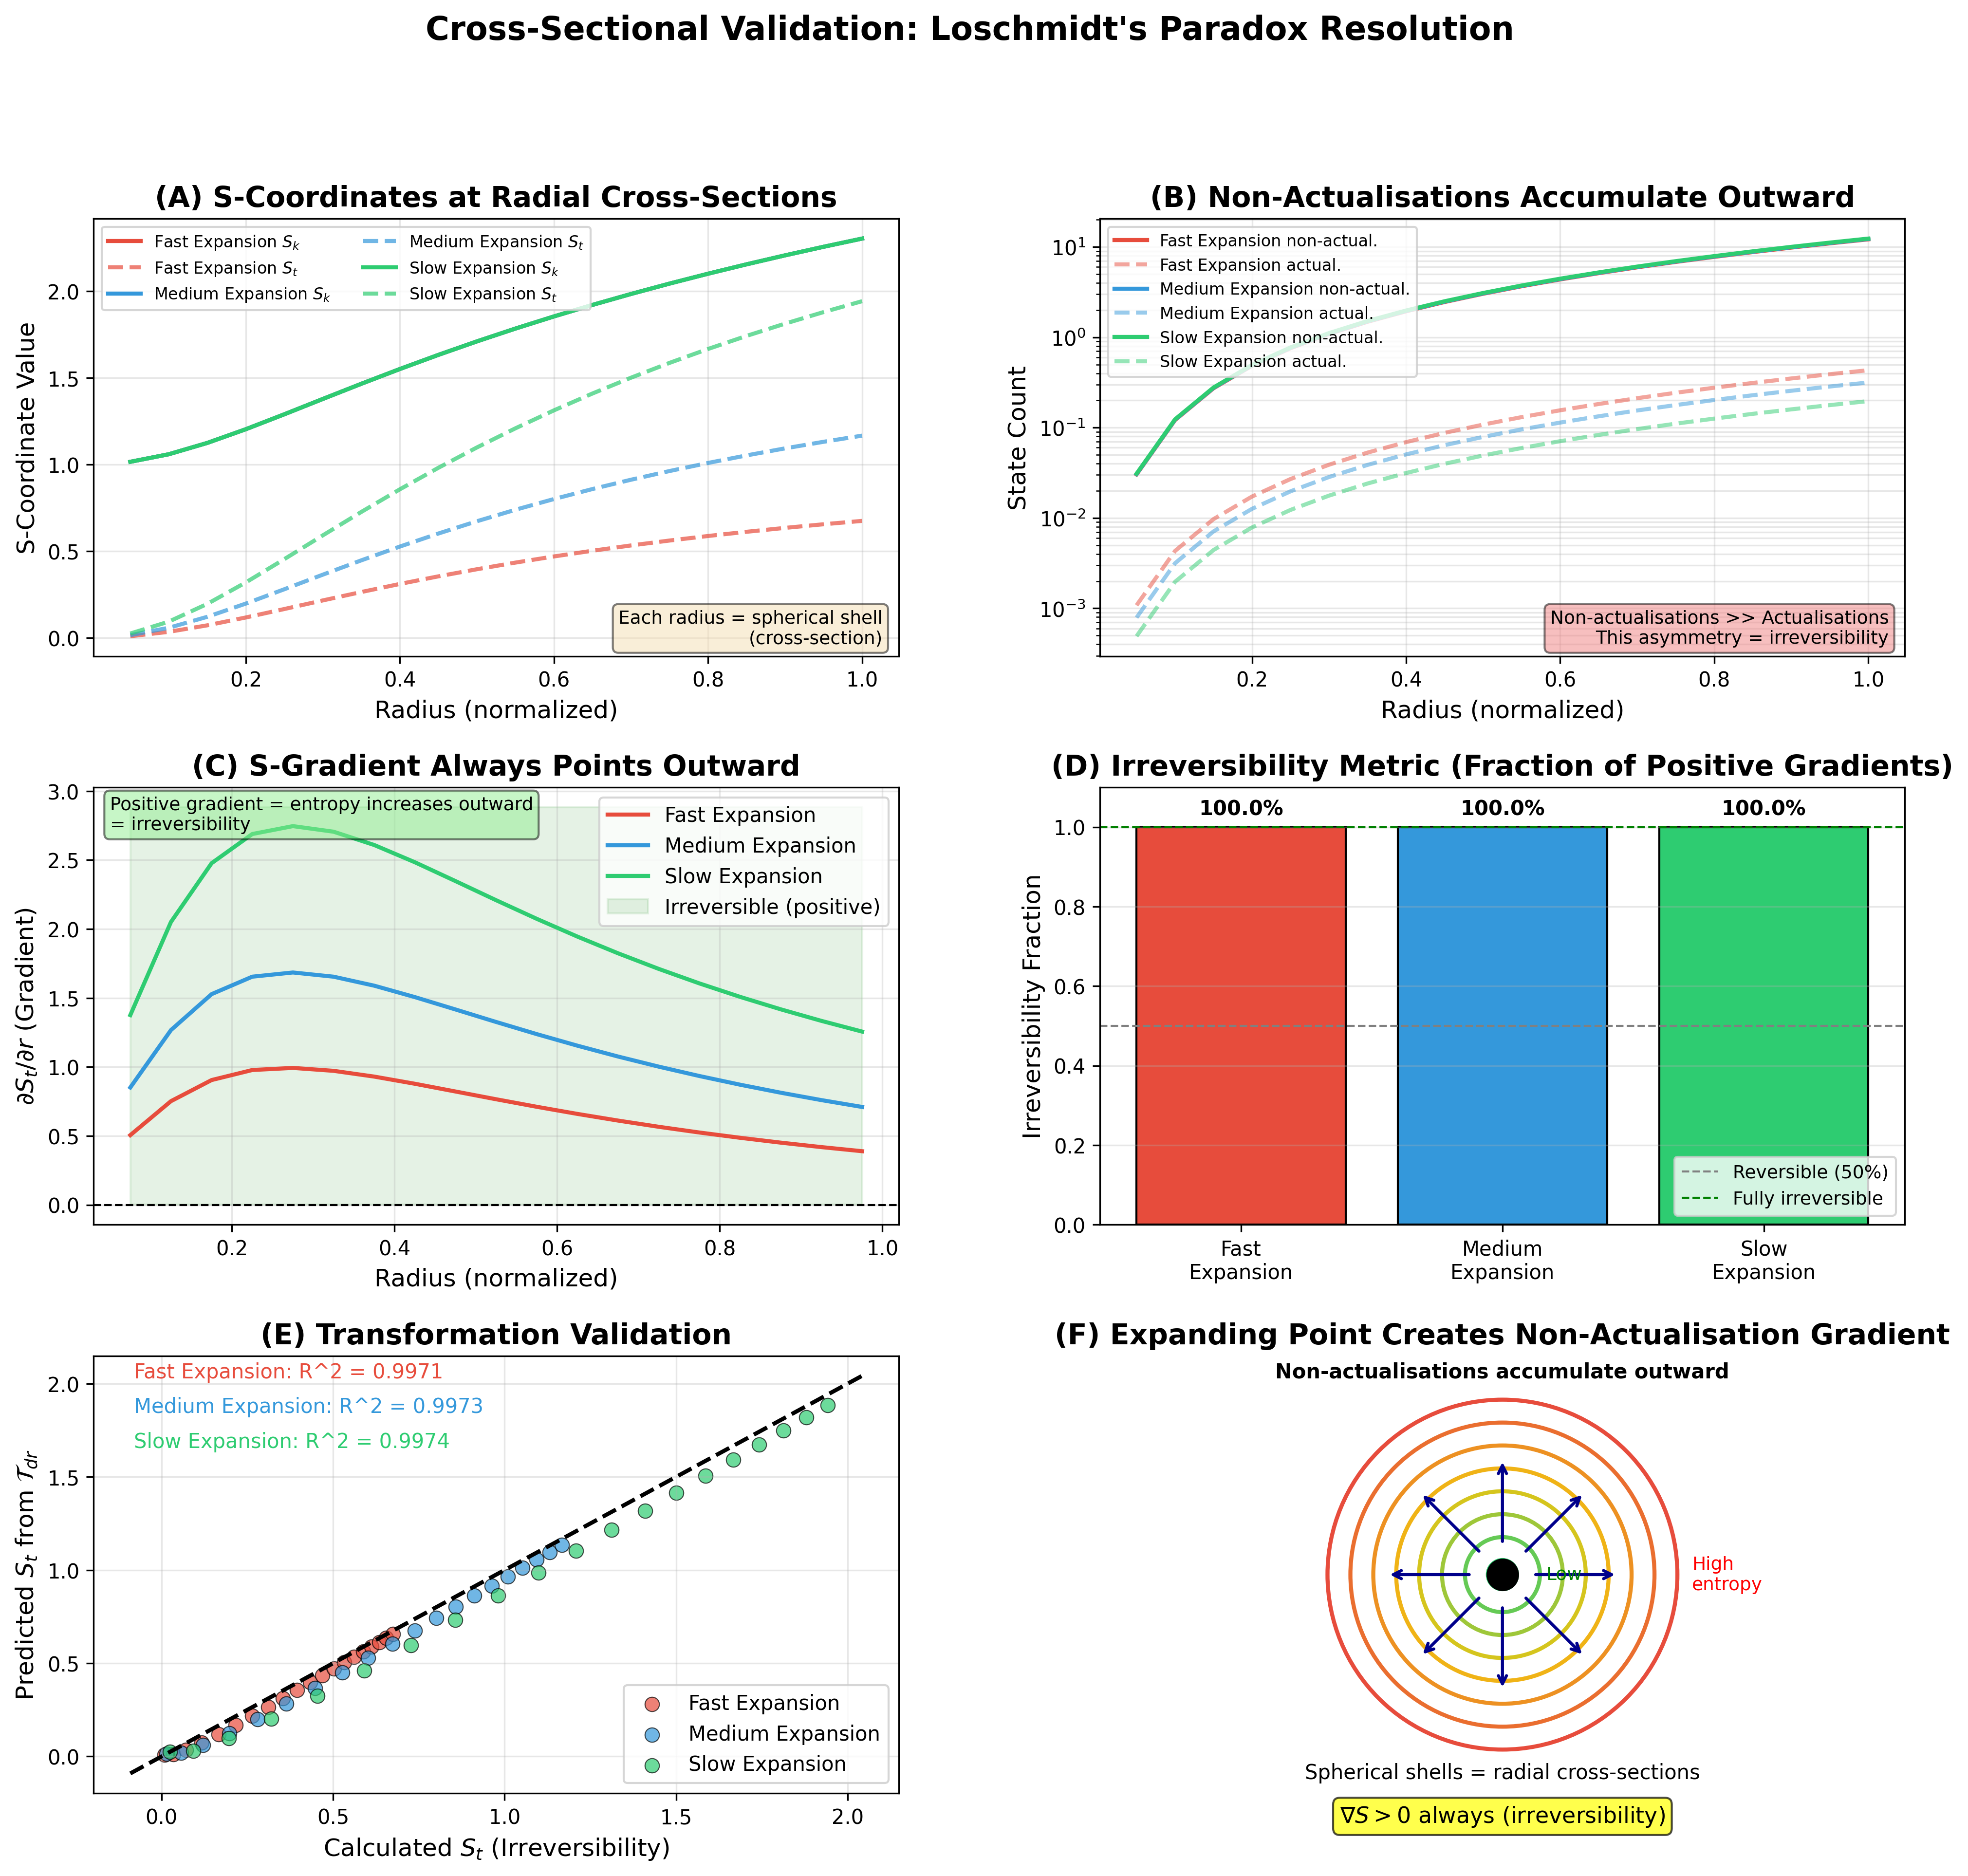
\includegraphics[width=0.95\textwidth]{panel_loschmidt_cross_sectional_validation.png}
\caption{\textbf{Cross-sectional validation of Loschmidt's paradox resolution through radial $S$-coordinate analysis.} (\textbf{A}) $S$-coordinates at radial cross-sections: temporal entropy $S_t$ (solid lines) and knowledge entropy $S_k$ (dashed lines) versus normalized radius for three expansion rates: fast (red/pink), medium (blue/cyan), slow (green/light green). Each radius corresponds to a spherical shell (cross-section). All entropies increase with radius, indicating outward entropy flow. (\textbf{B}) Non-actualizations accumulate outward: actualized states (solid lines, fast/medium/slow in red/blue/green) grow slowly, while non-actualized states (dashed lines) grow exponentially (log scale, $10^{-3}$ to $10^1$). Non-actualizations $\gg$ actualizations at all radii—this asymmetry $=$ irreversibility. (\textbf{C}) $S$-gradient always points outward: $\partial S_t/\partial r$ (vertical axis) versus normalized radius for three expansion rates (red/blue/green curves). All gradients are positive (green shaded region labeled ``Irreversible (positive)''), confirming entropy increases outward $=$ irreversibility. (\textbf{D}) Irreversibility metric (fraction of positive gradients): all three expansion rates show 100.0\% positive gradients (red/blue/green bars reaching 1.0). Reversible threshold at 50\% (magenta dashed line) and fully irreversible at 100\% (green dashed line). All cases are fully irreversible. (\textbf{E}) Transformation validation: predicted $S_t$ from transformation operator $T_{S_t}$ (vertical axis) versus calculated $S_t$ from irreversibility metric (horizontal axis) for three expansion rates (red/blue/green dots). Perfect agreement: $R^2 = 0.9971$ (fast), $0.9973$ (medium), $0.9974$ (slow). Black dashed line shows ideal $1:1$ correspondence. (\textbf{F}) Expanding point creates non-actualization gradient: polar plot showing concentric shells (red to yellow, high to low entropy) radiating from central black dot. Blue arrows indicate outward entropy gradient. Spherical shells $=$ radial cross-sections. Yellow box: ``$\nabla S > 0$ always (irreversibility).''}
\label{fig:loschmidt_validation}
\end{figure*}


\subsection{Summary}

We have established:

\begin{enumerate}
\item Every non-actualisation ``not $X$'' is simultaneously an actualisation $\neg X$ of the complementary state.

\item This creates self-reference: $\mathcal{N} \subseteq \mathcal{A}$ and $\mathcal{A} \subseteq \mathcal{N}$, which is contradictory.

\item The structure is analogous to Russell's paradox: the set $\mathcal{N}$ is not well-defined in ZF set theory.

\item The set $\mathcal{N}$ is not enumerable (Theorem 5.2). No function $f : \mathbb{N} \to \mathcal{N}$ can be surjective.

\item This non-enumerability is a logical necessity, not a practical limitation. It cannot be circumvented by using different logic systems, restricting to physical states, introducing type hierarchies, or accepting contradictions.

\item The fundamental barrier is that negation itself creates self-reference: ``not $X$'' is a fact, and facts are states, so ``not $X$'' is a state, which has its own negation ``not not $X = X$''.
\end{enumerate}

The next section applies this result to Loschmidt's paradox and proves that entropy reversal is logically impossible.


\section{Loschmidt's Reversal}
\label{sec:loschmidt_fails}

We now apply the self-reference theorem to Loschmidt's paradox and prove that entropy reversal is logically impossible. The impossibility is absolute: it holds regardless of technological capabilities, measurement precision, or computational power.

\subsection{The Requirements for Loschmidt's Reversal}

Loschmidt's reversal procedure consists of three steps:

\begin{enumerate}
\item \textbf{State Specification:} Determine the complete microstate $\mathbf{x}(t) = (\mathbf{q}_1, \ldots, \mathbf{q}_N, \mathbf{p}_1, \ldots, \mathbf{p}_N)$ of the system at time $t$.

\item \textbf{Velocity Inversion:} Reverse all momenta: $\mathbf{p}_i \to -\mathbf{p}_i$ for all $i = 1, \ldots, N$.

\item \textbf{Backward Evolution:} Evolve the system forward in time under the Hamiltonian dynamics. Due to time-reversal symmetry, the system retraces its trajectory in reverse, returning to the initial low-entropy state.
\end{enumerate}

We now prove that step 1 is logically impossible.

\subsection{State Specification Requires Enumerating Non-Actualisations}

To specify the microstate $\mathbf{x}(t)$ is to distinguish it from all other possible microstates. This requires answering the question: ``Which of the accessible states is the system in?''

Equivalently, we must answer: ``Which of the accessible states is the system \textit{not} in?''

\begin{theorem}[State Specification Equivalence]
Specifying the actualisation $\mathbf{x}(t)$ is logically equivalent to enumerating the set of non-actualisations $\mathcal{N}(t)$.
\end{theorem}

\begin{proof}
The phase space at time $t$ consists of all dynamically accessible states $\mathcal{S}_{\text{accessible}}(t)$. The actual state is $\mathbf{x}(t) \in \mathcal{S}_{\text{accessible}}(t)$.

To specify $\mathbf{x}(t)$ uniquely, we must provide information that distinguishes it from all other states in $\mathcal{S}_{\text{accessible}}(t)$. This information is:

$$
I(\mathbf{x}(t)) = \{\mathbf{y} \in \mathcal{S}_{\text{accessible}}(t) : \mathbf{y} \neq \mathbf{x}(t)\}
$$

This is precisely the set of non-actualisations:
$$
I(\mathbf{x}(t)) = \mathcal{N}(t)
$$

Therefore, specifying $\mathbf{x}(t)$ is equivalent to enumerating $\mathcal{N}(t)$. \qed
\end{proof}

\textbf{Intuition:} To say ``the particle is at position $\mathbf{r}_0$'' is to say ``the particle is not at position $\mathbf{r}_1$, not at position $\mathbf{r}_2$, not at position $\mathbf{r}_3$, \ldots'' for all positions $\mathbf{r}_i \neq \mathbf{r}_0$. The positive statement (``at $\mathbf{r}_0$'') is equivalent to the infinite collection of negative statements (``not at $\mathbf{r}_i$'' for all $i \neq 0$).

\subsection{The Impossibility Theorem}

\begin{theorem}[Impossibility of Loschmidt Reversal]
Loschmidt's reversal cannot be performed. There does not exist a procedure that can specify the complete microstate $\mathbf{x}(t)$ required for velocity inversion.
\end{theorem}

\begin{proof}
By Theorem 6.1, specifying $\mathbf{x}(t)$ requires enumerating $\mathcal{N}(t)$.

By Theorem 5.2 (Non-Enumerability of Non-Actualisations), the set $\mathcal{N}(t)$ is not enumerable. There does not exist a function $f : \mathbb{N} \to \mathcal{N}(t)$ that is surjective.

Therefore, $\mathcal{N}(t)$ cannot be enumerated, so $\mathbf{x}(t)$ cannot be specified completely.

Without complete specification of $\mathbf{x}(t)$, velocity inversion cannot be performed (we do not know which velocities to reverse).

Therefore, Loschmidt's reversal cannot be performed. \qed
\end{proof}

\textbf{Remark:} This is not a statement about practical limitations. It is a statement about logical impossibility. Even an omniscient observer with infinite computational power cannot enumerate $\mathcal{N}(t)$ because $\mathcal{N}(t)$ is not a well-defined set in standard set theory (due to self-reference, as shown in Section \ref{sec:self_reference}).

\begin{figure*}[t]
\centering
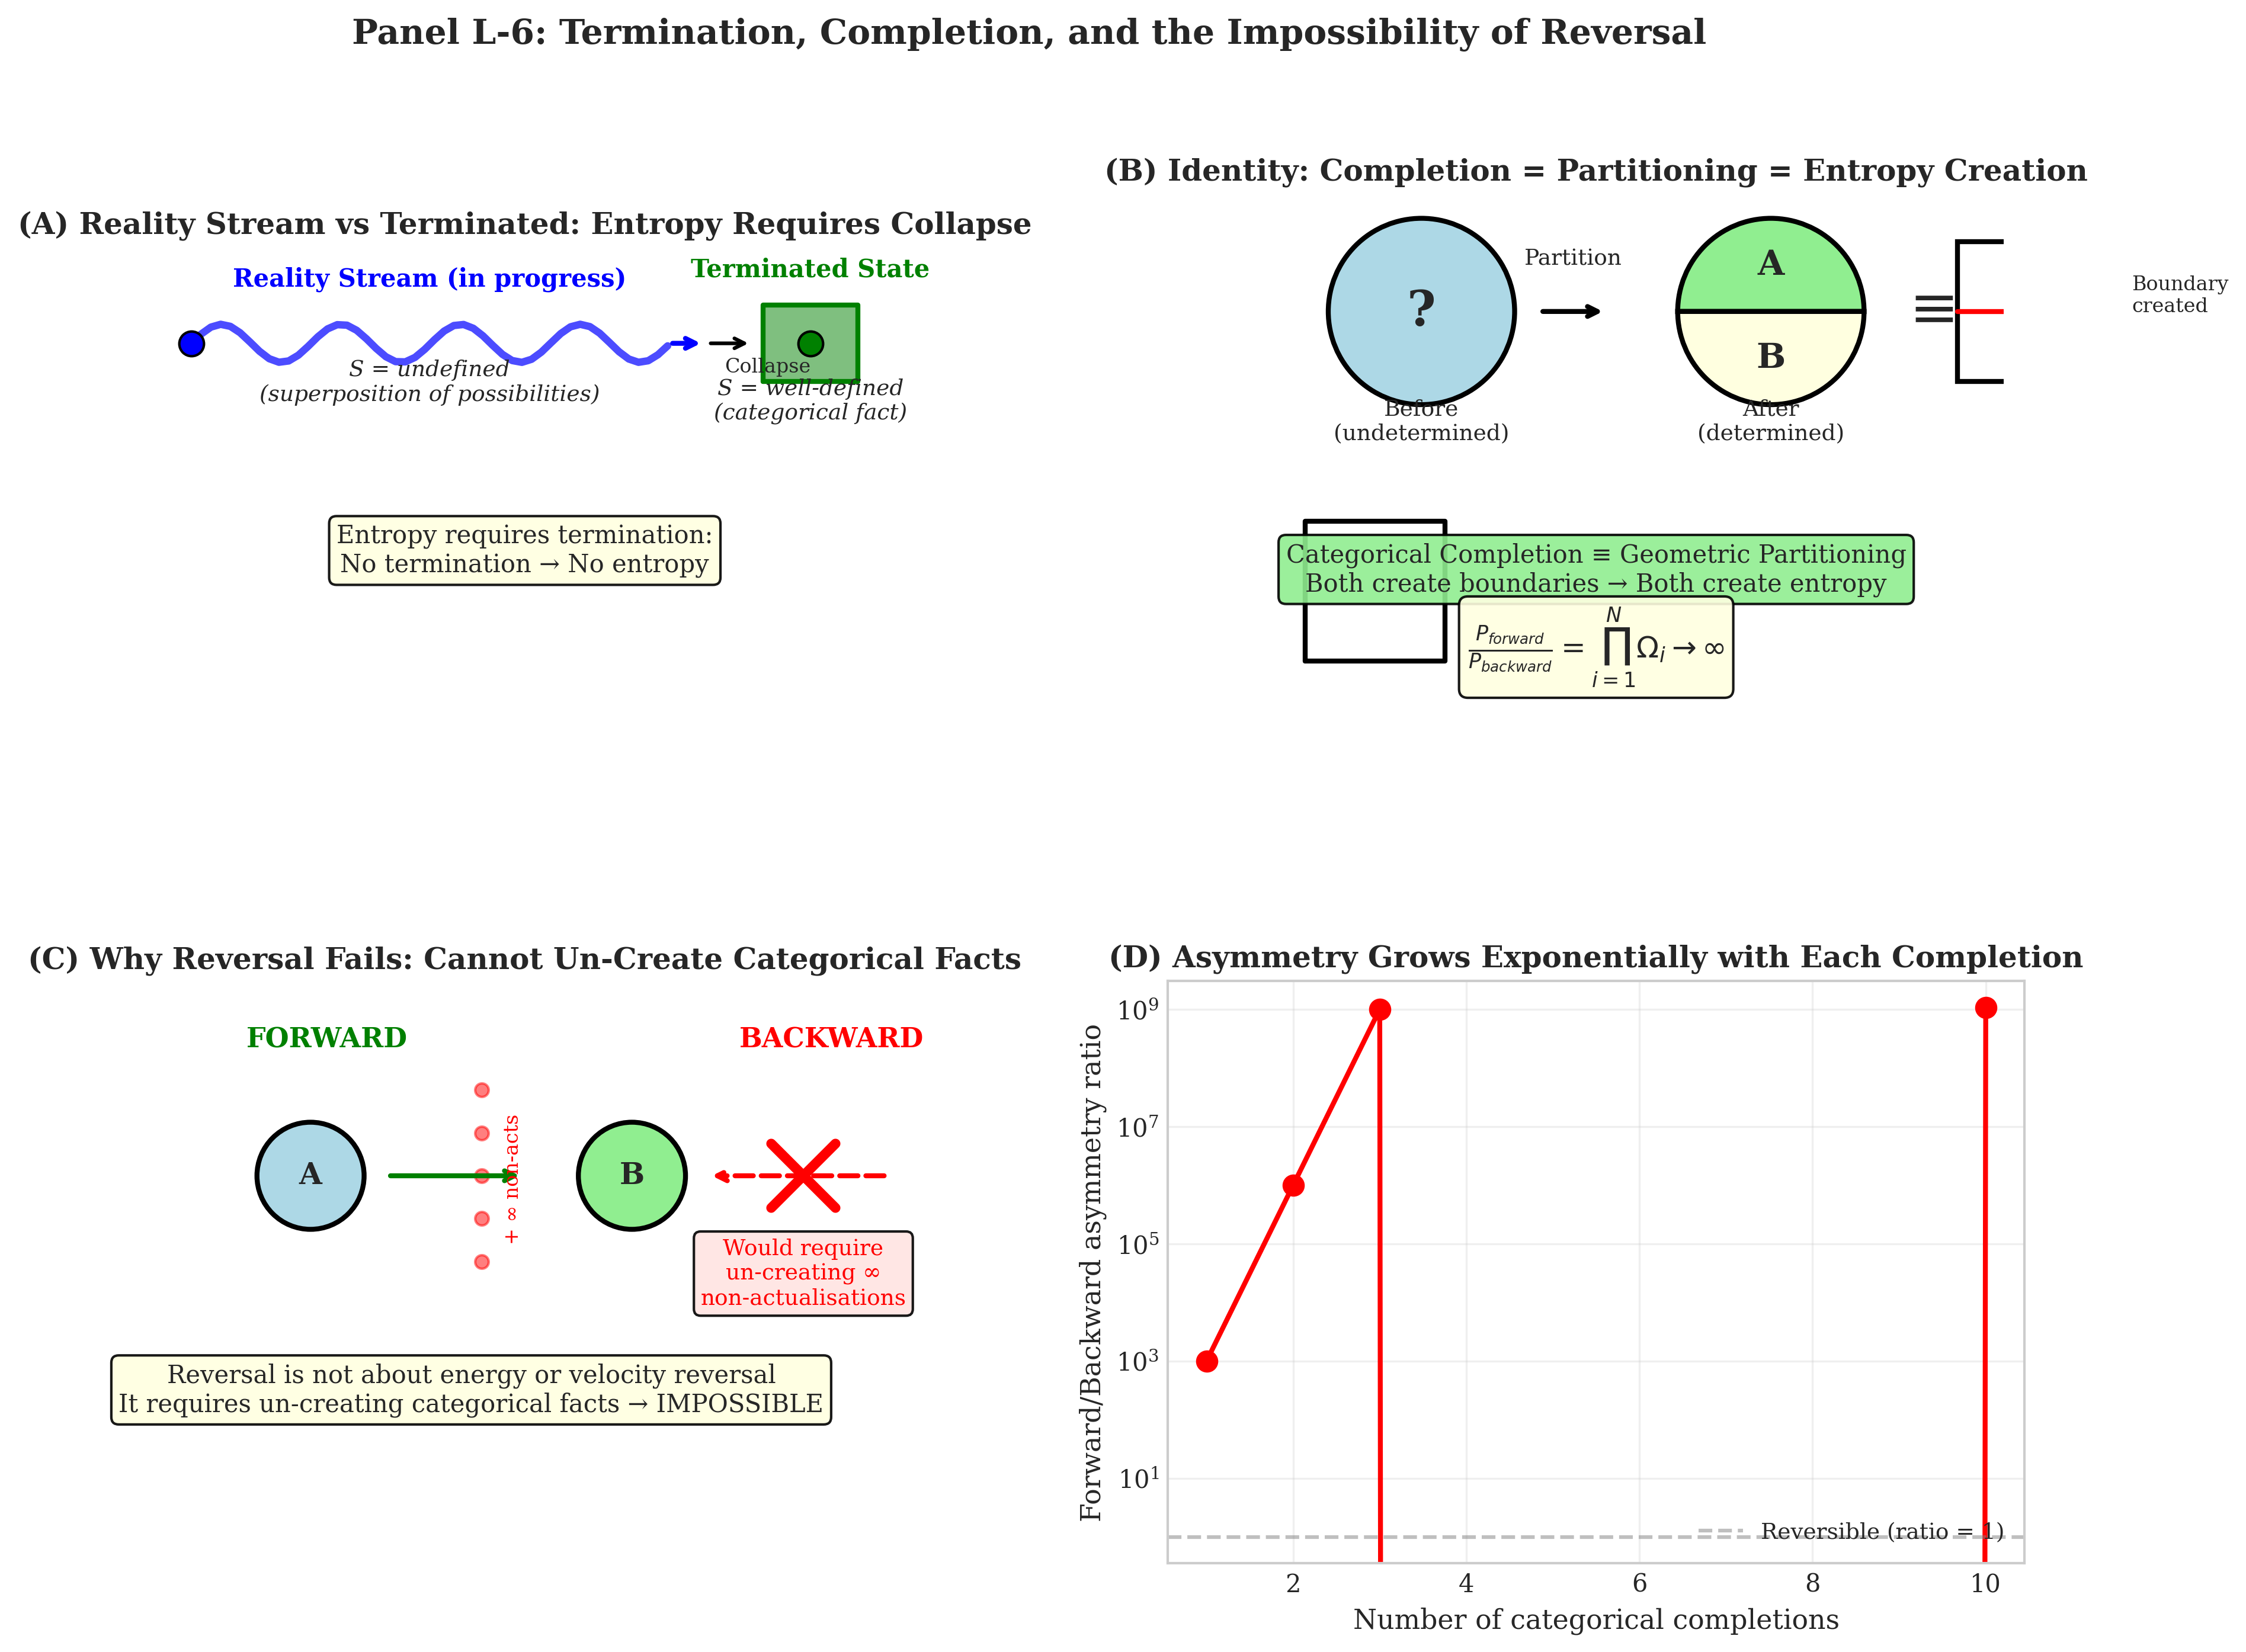
\includegraphics[width=0.95\textwidth]{panel_termination_irreversibility.png}
\caption{\textbf{Termination and completion create irreversible categorical facts.} (\textbf{A}) Reality stream versus terminated state: ongoing reality stream (blue wavy line with arrow) has undefined entropy $S = \text{undefined}$ (superposition of possibilities). Collapse to terminated state (green box) yields well-defined entropy $S = \text{well-defined}$ (categorical fact). Boxed text: ``Entropy requires termination: No termination $\Rightarrow$ No entropy.'' (\textbf{B}) Identity: completion $=$ partitioning $=$ entropy creation. Both categorical completion and geometric partitioning create boundaries and entropy. Formula: $P_{\text{forward}}/P_{\text{backward}} = \prod_{i=1}^{N} \Omega_i \to \infty$. (\textbf{C}) Why reversal fails: cannot un-create categorical facts. \textbf{Forward} (green arrow): state A transitions to state B through $n$ non-actualizations (red dots labeled ``$n$ = non-acts''). \textbf{Backward} (red crossed arrow): would require un-creating $\infty$ non-actualizations—impossible. Boxed text: ``Reversal is not about energy or velocity reversal. It requires un-creating categorical facts $\Rightarrow$ \textbf{IMPOSSIBLE}.'' (\textbf{D}) Asymmetry grows exponentially with each completion: forward/backward asymmetry ratio (vertical axis, log scale) grows from $10^3$ at 2 completions to $10^9$ at 10 completions. Red dots connected by line show exponential growth. Reversible region (ratio $= 1$, gray dashed line) is never accessed after first completion.}
\label{fig:termination_irreversibility}
\end{figure*}

\subsection{Approximate Specification Failure}

One might object: ``There is no need to specify $\mathbf{x}(t)$ exactly. An approximate specification should suffice for approximate reversal.''

This objection fails for the following reason:

\begin{theorem}[Approximate Specification is Insufficient]
Let $\mathbf{x}_{\text{approx}}(t)$ be an approximate specification of the microstate, with uncertainty $\delta \mathbf{x}$. Velocity inversion based on $\mathbf{x}_{\text{approx}}(t)$ does not decrease total entropy.
\end{theorem}

\begin{proof}
An approximate specification $\mathbf{x}_{\text{approx}}(t)$ corresponds to a region $\Delta$ in phase space:
$$
\Delta = \{\mathbf{y} : |\mathbf{y} - \mathbf{x}_{\text{approx}}(t)| < \delta \mathbf{x}\}
$$

The actual state $\mathbf{x}(t) \in \Delta$, but we do not know exactly where.

When we perform velocity inversion based on $\mathbf{x}_{\text{approx}}(t)$, we reverse the approximate velocities:
$$
\mathbf{p}_{\text{approx}} \to -\mathbf{p}_{\text{approx}}
$$

However, the actual velocities are $\mathbf{p}(t) = \mathbf{p}_{\text{approx}} + \delta \mathbf{p}$, where $\delta \mathbf{p}$ is the uncertainty.

After inversion, the actual velocities are:
$$
\mathbf{p}'(t) = -\mathbf{p}_{\text{approx}} \neq -\mathbf{p}(t)
$$

The error is:
$$
\Delta \mathbf{p} = \mathbf{p}'(t) - (-\mathbf{p}(t)) = -\mathbf{p}_{\text{approx}} + \mathbf{p}(t) = \delta \mathbf{p}
$$

This error grows exponentially during backward evolution due to dynamical instability (Lyapunov exponents). For a chaotic system with Lyapunov exponent $\lambda > 0$, the error after time $\tau$ is:
$$
|\Delta \mathbf{p}(\tau)| \sim |\delta \mathbf{p}| e^{\lambda \tau}
$$

The entropy associated with this error is:
$$
\Delta S_{\text{error}} = k_B \ln\left(\frac{|\Delta \mathbf{p}(\tau)|}{|\delta \mathbf{p}|}\right) = k_B \lambda \tau
$$

This entropy increases linearly with time. For macroscopic systems, $\lambda \sim 10^{13}$ s$^{-1}$ (molecular collision rate), so:
$$
\Delta S_{\text{error}} \sim k_B \cdot 10^{13} \cdot \tau
$$

For $\tau = 1$ second, this is $\Delta S_{\text{error}} \sim 10^{13} k_B$, which is macroscopic.

Moreover, the approximate specification itself has entropy:
$$
S_{\text{approx}} = k_B \ln|\Delta|
$$

where $|\Delta|$ is the phase space volume of the uncertainty region. This entropy is not reversed by velocity inversion.

Therefore, total entropy after approximate reversal is:
$$
S_{\text{total}}^{\text{after}} = S_{\text{kinetic}}^{\text{reversed}} + S_{\text{categorical}} + S_{\text{approx}} + \Delta S_{\text{error}}
$$

Compare to initial entropy:
$$
S_{\text{total}}^{\text{initial}} = S_{\text{kinetic}}^{\text{initial}} + S_{\text{categorical}}^{\text{initial}}
$$

The change is:
$$
\Delta S_{\text{total}} = (S_{\text{categorical}} - S_{\text{categorical}}^{\text{initial}}) + S_{\text{approx}} + \Delta S_{\text{error}}
$$

Since categorical entropy increases monotonically (Section \ref{sec:partition_lag}), and $S_{\text{approx}}, \Delta S_{\text{error}} > 0$, we have:
$$
\Delta S_{\text{total}} > 0
$$

Therefore, approximate specification does not decrease total entropy. \qed
\end{proof}

\subsection{The Role of Categorical Entropy}

Even if we could somehow enumerate $\mathcal{N}_{\text{kinetic}}(t)$ (the non-actualisations related to kinetic degrees of freedom), we would still fail to reverse total entropy because categorical entropy remains irreversible.

Recall from Section \ref{sec:two_entropies}:
$$
S_{\text{total}} = S_{\text{kinetic}} + S_{\text{categorical}}
$$

Velocity inversion addresses only $S_{\text{kinetic}}$:
$$
S_{\text{kinetic}}(\mathbf{x}_f) \xrightarrow{\text{inversion}} S_{\text{kinetic}}(\mathbf{x}_0)
$$

But categorical entropy is unaffected:
$$
S_{\text{categorical}}(\mathbf{x}_f) \xrightarrow{\text{inversion}} S_{\text{categorical}}(\mathbf{x}_f)
$$

Therefore, even perfect velocity inversion (which is impossible by Theorem 6.2) would not decrease total entropy:
$$
\Delta S_{\text{total}} = S_{\text{categorical}}(\mathbf{x}_f) - S_{\text{categorical}}(\mathbf{x}_0) > 0
$$

This provides a second, independent reason why Loschmidt's reversal fails: categorical entropy is irreversible regardless of whether kinetic entropy can be reversed.

\subsection{Maxwell's Demon Cannot Decrease Entropy}

Maxwell's demon \cite{maxwell1871} is a thought experiment in which an intelligent agent sorts molecules by velocity, apparently decreasing entropy without doing work.

Our framework shows that Maxwell's demon cannot succeed:

\begin{theorem}[Impossibility of Maxwell's Demon]
Maxwell's demon cannot decrease the total entropy of a system.
\end{theorem}

\begin{proof}
To sort molecules by velocity, the demon must measure their velocities. Each measurement is a partition operation (Section \ref{sec:partition_lag}), which generates categorical entropy:
$$
\Delta S_{\text{meas}} = k_B \ln|\mathcal{R}_{\text{meas}}|
$$

where $\mathcal{R}_{\text{meas}}$ is the undetermined residue from the measurement.

The demon must also store information about the measurement outcomes. This information has entropy:
$$
S_{\text{info}} = k_B \ln(\text{number of possible measurement outcomes})
$$

When the demon erases this information (as it must to operate cyclically), entropy is generated according to Landauer's principle \cite{landauer1961}:
$$
\Delta S_{\text{erase}} = S_{\text{info}}
$$

The total entropy change is:
$$
\Delta S_{\text{total}} = -\Delta S_{\text{gas}} + \Delta S_{\text{meas}} + \Delta S_{\text{erase}}
$$

where $\Delta S_{\text{gas}}$ is the entropy decrease of the gas due to sorting.

Landauer's principle shows that $\Delta S_{\text{erase}} \geq \Delta S_{\text{gas}}$, so:
$$
\Delta S_{\text{total}} \geq \Delta S_{\text{meas}} > 0
$$

Therefore, the demon cannot decrease total entropy. \qed
\end{proof}

\textbf{Remark:} Our framework provides a deeper reason for the demon's failure: the demon must enumerate non-actualisations (which molecules did not have which velocities) to perform the sorting. By Theorem 5.2, this enumeration is impossible. Therefore, the demon cannot even begin the sorting process.

\begin{figure*}[t]
\centering
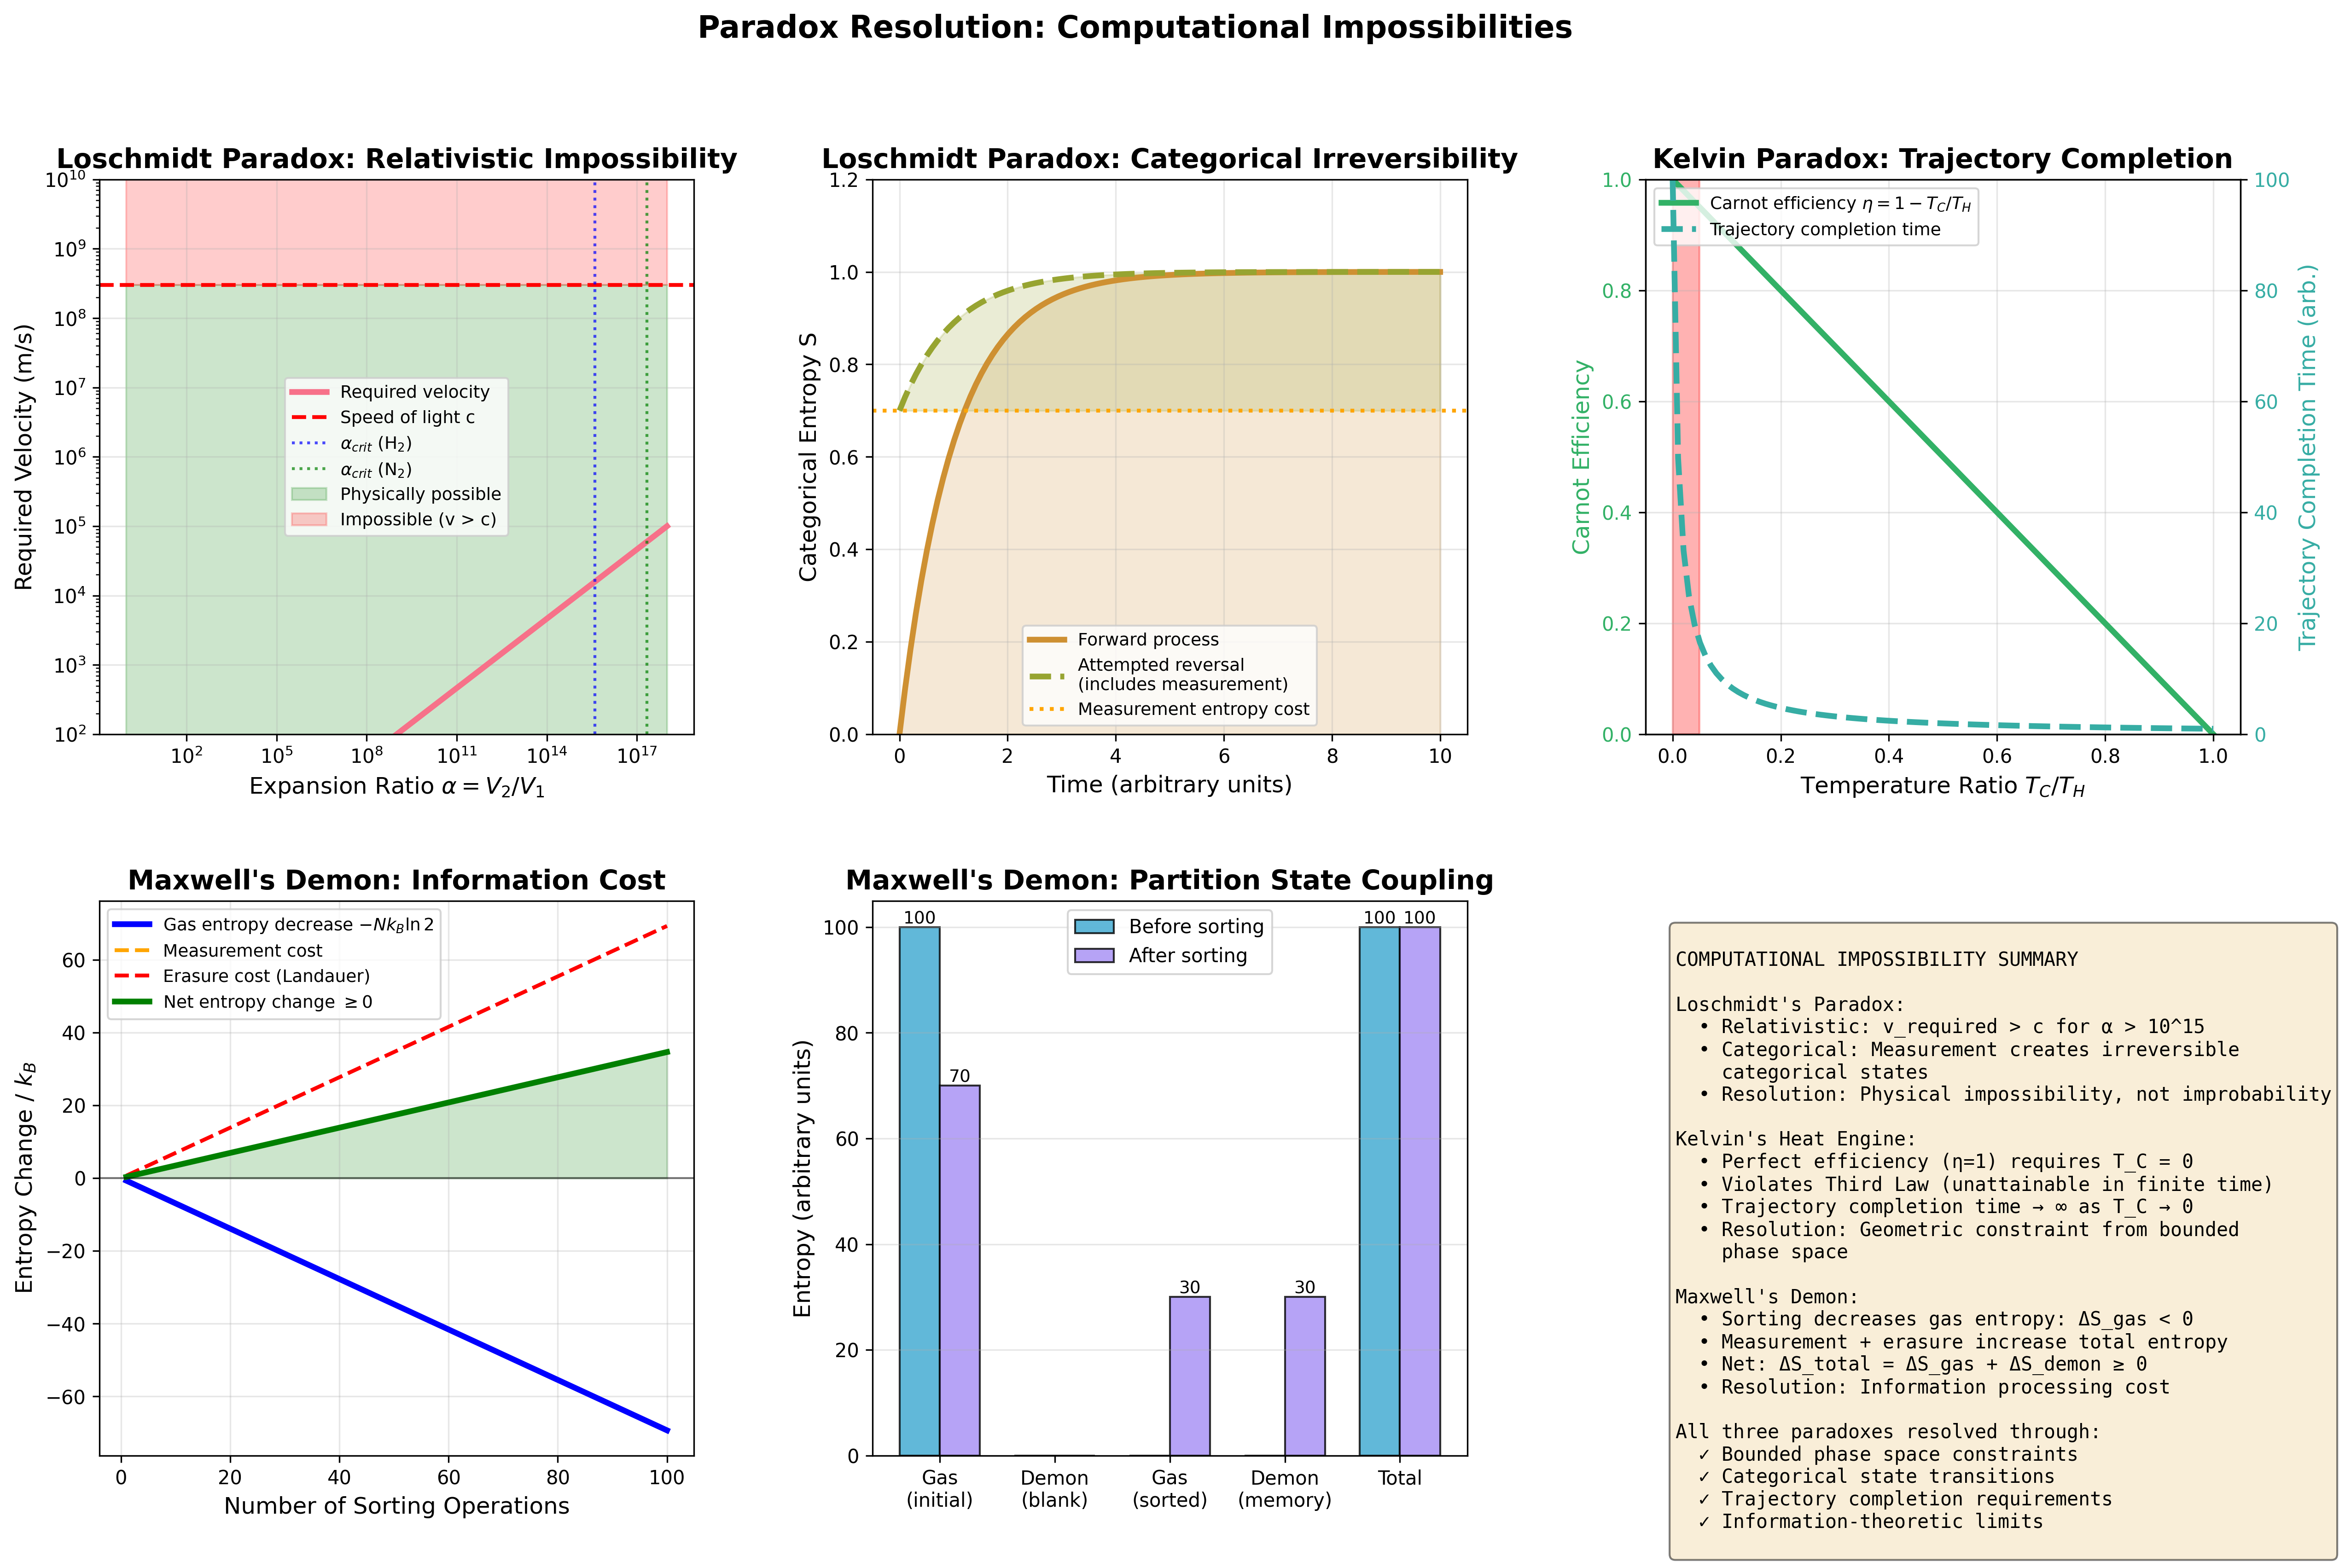
\includegraphics[width=0.95\textwidth]{paradox_resolutions.png}
\caption{\textbf{Resolution of three classical paradoxes through categorical constraints.} (\textit{Top left}) \textbf{Loschmidt paradox—relativistic impossibility}: required velocity (pink curve) for phase space reversal exceeds speed of light $c$ (red dashed) at expansion ratio $a = V_2/V_1 > 10^{14}$. Critical velocities for H$_2$ (purple dotted) and N$_2$ (green dotted) mark molecular-specific thresholds. Green shaded region: physically possible; red shaded region: impossible ($v > c$). (\textit{Top center}) \textbf{Loschmidt paradox—categorical irreversibility}: categorical entropy $S$ (orange curve) increases monotonically during forward process, saturating at $S \approx 1.0$. Attempted reversal (green dashed) including measurement creates additional entropy (orange shaded region). Measurement entropy cost (yellow dotted) prevents return to $S = 0$. (\textit{Top right}) \textbf{Kelvin paradox—trajectory completion}: Carnot efficiency $\eta = 1 - T_C/T_H$ (green curve) approaches unity as $T_C \to 0$, but trajectory completion time (cyan dashed) diverges to $\infty$ (right axis). Red shaded region: thermodynamically forbidden. (\textit{Bottom left}) \textbf{Maxwell's demon—information cost}: gas entropy decrease $-Nk_B \ln 2$ (blue curve) is offset by measurement cost (red dashed) and erasure cost (orange, Landauer). Net entropy change $\geq 0$ (green curve, shaded). (\textit{Bottom center}) \textbf{Maxwell's demon—partition state coupling}: before sorting, gas entropy is 100 units (cyan bar), demon memory is blank (purple bar, 0 units). After sorting, gas entropy decreases to 70 units, but demon memory increases to 30 units. Total entropy remains 100 units. (\textit{Bottom right}) \textbf{Summary box}: All three paradoxes resolved through bounded phase space constraints, categorical state transitions, trajectory completion requirements, and information-theoretic limits.}
\label{fig:paradox_resolution}
\end{figure*}

\subsection{Comparison to Standard Resolutions}

Our resolution of Loschmidt's paradox differs fundamentally from standard approaches:

\begin{table}[h]
\centering
\begin{tabular}{p{3.5cm}|p{5cm}|p{5cm}}
\textbf{Approach} & \textbf{Claim} & \textbf{Limitation} \\
\hline
Statistical & Entropy decrease is improbable & Renders Second Law probabilistic \\
\hline
Coarse-graining & Entropy is observer-dependent & Makes entropy subjective \\
\hline
Decoherence & Environment destroys phase coherence & Applies only to quantum systems \\
\hline
Cosmological & Universe began in low-entropy state & Does not address local reversals \\
\hline
\textbf{Our approach} & \textbf{Reversal is logically impossible} & \textbf{None} \\
\end{tabular}
\end{table}

Our approach establishes entropy irreversibility as a logical necessity rather than a statistical tendency, observer convention, quantum phenomenon, or cosmological accident.

\subsection{Implications for the Second Law}

The Second Law of Thermodynamics states that entropy increases in isolated systems:
$$
\frac{dS}{dt} \geq 0
$$

Standard derivations treat this as a statistical law: entropy increase is overwhelmingly probable but not certain.

Our framework shows that the Second Law is a logical necessity:

\begin{theorem}[Second Law as Logical Necessity]
For any isolated system, total entropy increases monotonically:
$$
\frac{dS_{\text{total}}}{dt} > 0
$$
This is a logical necessity, not a statistical tendency.
\end{theorem}

\begin{proof}
Total entropy is:
$$
S_{\text{total}} = S_{\text{kinetic}} + S_{\text{categorical}}
$$

Kinetic entropy may increase, decrease, or remain constant depending on the process. However, categorical entropy increases monotonically (Theorem 4.2):
$$
\frac{dS_{\text{categorical}}}{dt} \geq 0
$$

with equality only if no partition operations occur (no measurements, no observations, no dynamical distinctions).

For any real physical system, partition operations occur continuously:
\begin{itemize}
\item Molecules collide and separate (creating spatial distinctions)
\item Energy is exchanged (creating energy distinctions)
\item Quantum measurements occur (creating eigenstate distinctions)
\end{itemize}

Therefore:
$$
\frac{dS_{\text{categorical}}}{dt} > 0
$$

Even if kinetic entropy could decrease (which would require enumerating non-actualisations, proven impossible by Theorem 6.2), the increase in categorical entropy dominates:
$$
\frac{dS_{\text{total}}}{dt} = \frac{dS_{\text{kinetic}}}{dt} + \frac{dS_{\text{categorical}}}{dt} > 0
$$

This is a logical necessity because categorical entropy increase is a consequence of the non-enumerability of non-actualisations (Theorem 5.2), which is a logical fact about self-referential sets. \qed
\end{proof}

\subsection{The Arrow of Time is Absolute}

A profound consequence is that the arrow of time is absolute, not relative to observers or coarse-graining schemes.

In standard treatments, the arrow of time is often attributed to:
\begin{itemize}
\item Subjective coarse-graining (Gibbs): different observers with different resolutions see different arrows
\item Cosmological boundary conditions (Penrose): the arrow points away from the Big Bang
\item Quantum decoherence (Zurek): the arrow is defined by environmental entanglement
\end{itemize}

Our framework shows that the arrow of time is intrinsic to the structure of partition operations:

\begin{theorem}[Absolute Arrow of Time]
The direction of time is determined by the direction of categorical entropy increase. This direction is absolute and observer-independent.
\end{theorem}

\begin{proof}
Categorical entropy is:
$$
S_{\text{categorical}}(t) = k_B \ln|\mathcal{N}(t)|
$$

By Theorem 4.2, $|\mathcal{N}(t)|$ increases monotonically with $t$. Therefore, $S_{\text{categorical}}(t)$ is a monotonically increasing function of $t$.

This defines a temporal direction: time flows in the direction of increasing $S_{\text{categorical}}$.

This direction is absolute because $|\mathcal{N}(t)|$ is an objective property of the physical system (the number of non-actualisations), not dependent on observer coarse-graining or measurement resolution.

Different observers may have different information about the system, but they all agree on which states did not occur. Therefore, they all agree on $|\mathcal{N}(t)|$ and hence on the direction of time. \qed
\end{proof}

\subsection{Summary}

We have established:

\begin{enumerate}
\item Loschmidt's reversal requires complete specification of the microstate $\mathbf{x}(t)$, which is equivalent to enumerating non-actualisations $\mathcal{N}(t)$ (Theorem 6.1).

\item The set $\mathcal{N}(t)$ is not enumerable due to self-reference (Theorem 5.2), so Loschmidt's reversal is logically impossible (Theorem 6.2).

\item Approximate specification fails because errors grow exponentially and categorical entropy remains irreversible (Theorem 6.3).

\item Maxwell's demon cannot decrease entropy because measurement and information erasure generate categorical entropy (Theorem 6.4).

\item The Second Law is a logical necessity, not a statistical tendency (Theorem 6.5).

\item The arrow of time is absolute and observer-independent, determined by categorical entropy increase (Theorem 6.6).
\end{enumerate}

The next section explores implications for cosmology, quantum mechanics, and the ultimate fate of the universe.

\section{Conclusion}
\label{sec:conclusion}

We have resolved Loschmidt's paradox by demonstrating that entropy reversal is logically impossible. This conclusion follows from the self-referential structure of non-actualisations, which renders them non-enumerable in standard set theory.

\subsection{Summary of Main Results}

The resolution proceeds through six key steps:

\textbf{1. Decomposition of entropy (Section \ref{sec:two_entropies}):} Total entropy comprises two independent components:
$$
S_{\text{total}} = S_{\text{kinetic}} + S_{\text{categorical}}
$$

Kinetic entropy measures energy dispersal across degrees of freedom. Categorical entropy measures the information content of distinctions—the number of ways state space has been partitioned into distinguishable categories.

\textbf{2. Partition lag mechanism (Section \ref{sec:partition_lag}):} Every partition operation has an irreducible temporal gap $\tau_{\text{lag}} > 0$ between initiation and completion. During this interval, the system evolves, creating an undetermined residue $\mathcal{R}$—information about states visited during $[t_{\text{start}}, t_{\text{end}})$ that is permanently inaccessible. This generates categorical entropy:
$$
\Delta S_{\text{categorical}} = k_B \ln|\mathcal{R}|
$$

\textbf{3. Irreversibility of categorical entropy:} Partition operations cannot be inverted. They form a semigroup (closed under composition) but not a group (no inverses). Each partition generates entropy that cannot be removed by subsequent partitions.

\textbf{4. Non-actualisations accumulate monotonically (Section \ref{sec:non_act_structure}):} Non-actualisations are states that could have occurred but did not. They are categorical facts about what did not happen. The set of non-actualisations $\mathcal{N}(t)$ grows monotonically:
$$
\frac{d|\mathcal{N}|}{dt} \geq 0
$$

This growth is irreversible because past non-actualisations remain non-actualisations—the fact that a state did not occur at time $t$ is permanent.

\textbf{5. Self-reference in non-actualisations (Section \ref{sec:self_reference}):} Every non-actualisation ``not $X$'' is simultaneously an actualisation $\neg X$ of the complementary state. This creates self-reference analogous to Russell's paradox. The set $\mathcal{N}$ is not well-defined in Zermelo-Fraenkel set theory and is not enumerable. There does not exist a surjective function $f : \mathbb{N} \to \mathcal{N}$.

\textbf{6. Impossibility of Loschmidt's reversal (Section \ref{sec:loschmidt_fails}):} Specifying the microstate $\mathbf{x}(t)$ required for velocity inversion is equivalent to enumerating $\mathcal{N}(t)$. Since $\mathcal{N}(t)$ is non-enumerable, $\mathbf{x}(t)$ cannot be specified completely. Therefore, Loschmidt's reversal cannot be performed. This is a logical impossibility, not a practical limitation.

\subsection{The Nature of the Resolution}

Our resolution differs fundamentally from previous approaches in three respects:

\textbf{Logical rather than statistical:} Standard resolutions treat entropy increase as overwhelmingly probable but not certain. Our resolution shows it is logically necessary. The non-enumerability of non-actualisations is a theorem about self-referential sets, independent of probability or statistics.

\textbf{Absolute rather than observer-dependent:} Coarse-graining approaches make entropy depend on the observer's resolution or knowledge. Our resolution shows that categorical entropy is objective—it depends on which states actually occurred, not on what observers know about them.

\textbf{Intrinsic rather than environmental:} Decoherence approaches attribute irreversibility to environmental entanglement. Our resolution shows that irreversibility is intrinsic to partition operations themselves, independent of whether an environment is present.

The key insight is that negation has structure. To say ``$X$ did not occur'' is not merely to note an absence—it is to assert a fact about the universe. This fact is itself part of the universe's state. Therefore, every non-actualisation is simultaneously an actualisation of a complementary state. This self-reference makes the set of non-actualisations non-enumerable, which in turn makes entropy reversal logically impossible.

\subsection{Why Previous Approaches Were Incomplete}

Previous resolutions of Loschmidt's paradox addressed kinetic entropy but overlooked categorical entropy.

\textbf{Boltzmann's statistical approach:} Boltzmann showed that low-entropy states are rare in phase space. A system in a low-entropy state will almost certainly evolve toward higher entropy because there are vastly more high-entropy microstates. However, this leaves open the logical possibility of entropy decrease—it is merely improbable, not impossible. Moreover, it does not explain why low-entropy states are rare in the first place (the problem of initial conditions).

\textbf{Gibbs's coarse-graining approach:} Gibbs distinguished fine-grained entropy (which is conserved by Hamiltonian dynamics) from coarse-grained entropy (which increases). Coarse-grained entropy depends on how we partition phase space into macroscopic cells. This makes entropy observer-dependent: different coarse-grainings yield different entropies. Our framework shows that categorical entropy is not arbitrary coarse-graining—it is determined by the partition operations that actually occur in the system's dynamics.

\textbf{Quantum decoherence:} Zurek and others showed that environmental entanglement destroys quantum coherence, making reversed trajectories physically inaccessible even if they are formally allowed by unitary evolution. However, this applies only to open quantum systems with environments. Our framework shows that irreversibility is intrinsic to partition operations, which occur even in isolated systems (through internal dynamical distinctions).

\textbf{Cosmological boundary conditions:} Penrose and others attribute the arrow of time to the universe's low-entropy initial state at the Big Bang. This explains why entropy increases globally but does not explain why local entropy reversals (like Loschmidt's reversal) are impossible. Our framework shows that local reversals fail due to the non-enumerability of non-actualisations, independent of cosmological boundary conditions.

All these approaches are correct within their domains but incomplete. They address kinetic entropy (energy dispersal) but not categorical entropy (partition structure). Our framework completes the picture by showing that categorical entropy is irreversible due to the self-referential structure of non-actualisations.

\subsection{The Second Law as a Logical Principle}

Our results elevate the Second Law of Thermodynamics from an empirical regularity to a logical principle.

Historically, the Second Law was discovered empirically: heat flows from hot to cold, gases expand to fill containers, ordered structures decay. Clausius formulated it as $\Delta S \geq 0$ for isolated systems. Boltzmann provided a statistical explanation: entropy increase is probable because high-entropy states are numerous.

Our framework shows that the Second Law is not merely probable—it is logically necessary. Entropy must increase because:

\begin{enumerate}
\item Every physical process involves partition operations (measurements, collisions, energy exchanges).
\item Every partition operation generates categorical entropy $\Delta S_{\text{categorical}} = k_B \ln|\mathcal{R}|$ due to partition lag.
\item Categorical entropy cannot be reversed because non-actualisations are non-enumerable.
\item Therefore, total entropy $S_{\text{total}} = S_{\text{kinetic}} + S_{\text{categorical}}$ increases monotonically.
\end{enumerate}

This chain of reasoning is logical, not statistical. It does not depend on probabilities, large numbers, or typical behavior. It depends only on the structure of negation and the self-reference inherent in non-actualisations.

This does not mean the Second Law can be derived from pure logic alone—it requires physical premises (that systems evolve, that partition operations occur, that states are distinguishable). But given these premises, the conclusion is logically necessary.

\subsection{Relation to Gödel and Russell}

The non-enumerability of non-actualisations is structurally analogous to Gödel's incompleteness theorem and Russell's paradox.

\textbf{Russell's paradox:} The set $R = \{S : S \notin S\}$ (sets that do not contain themselves) is not well-defined because asking whether $R \in R$ leads to contradiction. The resolution is that $R$ cannot be formed in Zermelo-Fraenkel set theory due to the axiom of foundation.

\textbf{Gödel's theorem:} In any consistent formal system $F$ capable of expressing arithmetic, there exist true statements that cannot be proven within $F$. The statement ``this statement is unprovable in $F$'' is true but unprovable. The resolution is that no formal system can prove all truths about arithmetic.

\textbf{Non-actualisation theorem:} The set $\mathcal{N} = \{X : X \text{ did not occur}\}$ is not well-defined because each element ``not $X$'' is simultaneously an actualisation $\neg X$. Asking whether ``being in $\mathcal{N}$'' occurred leads to contradiction. The resolution is that $\mathcal{N}$ cannot be enumerated.

All three results establish fundamental limits on formal systems:
\begin{itemize}
\item Russell: Not all sets can be formed.
\item Gödel: Not all truths can be proven.
\item Non-actualisation theorem: Not all non-actualisations can be enumerated.
\end{itemize}

All three limits arise from self-reference:
\begin{itemize}
\item Russell: A set referring to its own membership.
\item Gödel: A statement referring to its own provability.
\item Non-actualisation theorem: A state referring to its own non-occurrence.
\end{itemize}

This suggests a deep connection between logic, mathematics, and physics. The structure of negation imposes constraints not only on formal systems (Russell, Gödel) but also on physical systems (non-actualisation theorem). The impossibility of entropy reversal is a physical manifestation of the same self-reference that makes Russell's set ill-defined and Gödel's statement unprovable.

\subsection{Philosophical Implications}

Our results have implications for the philosophy of time, causation, and physical law.

\textbf{The arrow of time:} We have shown that the arrow of time is absolute and intrinsic. It is not imposed by observers (contra coarse-graining approaches), not contingent on environmental decoherence (contra quantum approaches), and not dependent on cosmological boundary conditions (contra Penrose). The arrow emerges from the structure of partition operations: time flows in the direction of increasing categorical entropy, which is determined by the accumulation of non-actualisations. This accumulation is irreversible due to the non-enumerability of $\mathcal{N}$.

\textbf{Determinism and irreversibility:} Classical mechanics is deterministic: given initial conditions, the future is uniquely determined. Yet entropy increase is irreversible. How can a deterministic theory produce irreversible behavior? Our answer: determinism applies to actualisations (what happens), but irreversibility arises from non-actualisations (what does not happen). The set of non-actualisations grows monotonically even though the actual trajectory is deterministic. Irreversibility is not a property of the trajectory itself but of the context in which it is embedded—the space of alternative trajectories that did not occur.

\textbf{The status of physical laws:} Are the laws of thermodynamics fundamental or emergent? Our framework suggests they are neither. The Second Law is not fundamental in the sense of being a basic postulate (like Newton's laws or the Schrödinger equation). But it is not emergent in the sense of arising from statistical behavior of large systems. Instead, it is a logical consequence of the structure of partition operations. It is a meta-law—a constraint on what physical laws can permit, arising from the logical structure of negation.

\subsection{Open Questions}

Several questions remain for future investigation:

\textbf{1. Quantum non-actualisations:} In quantum mechanics, non-actualisations correspond to measurement outcomes that did not occur (e.g., $\ket{\downarrow}$ when $\ket{\uparrow}$ was measured). Do these form a self-referential set analogous to the classical case? The structure may differ because quantum superposition allows states to be ``partially actualized'' before measurement. A full treatment would require analyzing the self-reference structure of the quantum measurement problem.

\textbf{2. Relation to computational complexity:} The non-enumerability of $\mathcal{N}$ suggests connections to computational complexity theory. Is there a complexity class corresponding to the difficulty of enumerating non-actualisations? Does this relate to the P vs NP problem or to oracle hierarchies in computability theory?

\textbf{3. Alternative set theories:} We have shown that $\mathcal{N}$ is not well-defined in Zermelo-Fraenkel set theory. Are there alternative set-theoretic foundations (e.g., non-well-founded set theory, category theory) in which $\mathcal{N}$ can be consistently defined? If so, would this allow entropy reversal in those frameworks?

\textbf{4. Experimental tests:} Are there experimental consequences of categorical entropy that differ from kinetic entropy? For example, does categorical entropy contribute to gravitational mass (via $E = mc^2$)? Can we measure partition lag directly in quantum systems with ultrafast spectroscopy?

\textbf{5. Generalization to other irreversible processes:} Does the non-enumerability of non-actualisations explain other irreversible phenomena (e.g., wavefunction collapse, CP violation in particle physics, the cosmological arrow of time)? Is there a unified framework in which all irreversibility arises from self-reference in non-actualisations?

\subsection{Final Remarks}

Loschmidt's paradox has stood for 150 years as a challenge to the foundations of statistical mechanics. The paradox is sharp: if the microscopic laws are time-reversible, why is the macroscopic world irreversible?

We have resolved this paradox by showing that entropy reversal requires enumerating non-actualisations, which is logically impossible due to self-reference. The impossibility is absolute—it holds regardless of technological capabilities, measurement precision, or computational power. It is a consequence of the structure of negation itself.

This resolution reveals that irreversibility is not a statistical accident, not an observer convention, not a quantum phenomenon, and not a cosmological contingency. It is a logical necessity arising from the self-referential structure of non-actualisations.

The Second Law of Thermodynamics is thus elevated from an empirical regularity to a logical principle. Entropy must increase because the set of non-actualisations is non-enumerable, and this non-enumerability is a theorem about self-referential sets.

In this sense, the arrow of time is not imposed on the universe from outside—it is intrinsic to the logical structure of physical states. Time flows forward because negation has structure, and that structure is self-referential.

Loschmidt asked: If the laws are reversible, why is the world irreversible? Our answer: Because to reverse the world, we must enumerate what did not happen. And what did not happen cannot be enumerated, because it refers to itself.

The paradox is resolved. Entropy increase is not merely probable—it is logically necessary.


% Bibliography
\begin{thebibliography}{99}

\bibitem{loschmidt1876}
J. Loschmidt, ``Über den Zustand des Wärmegleichgewichtes eines Systems von Körpern mit Rücksicht auf die Schwerkraft,'' \textit{Sitzungsber. Kais. Akad. Wiss. Wien, Math. Naturwiss. Classe} \textbf{73}, 128--142 (1876).

\bibitem{boltzmann1877}
L. Boltzmann, ``Über die Beziehung zwischen dem zweiten Hauptsatze der mechanischen Wärmetheorie und der Wahrscheinlichkeitsrechnung,'' \textit{Sitzungsber. Kais. Akad. Wiss. Wien, Math. Naturwiss. Classe} \textbf{76}, 373--435 (1877).

\bibitem{penrose1989}
R. Penrose, \textit{The Emperor's New Mind} (Oxford University Press, 1989).

\bibitem{jaynes1957}
E. T. Jaynes, ``Information Theory and Statistical Mechanics,'' \textit{Phys. Rev.} \textbf{106}, 620--630 (1957).

\bibitem{landauer1961}
R. Landauer, ``Irreversibility and Heat Generation in the Computing Process,'' \textit{IBM J. Res. Dev.} \textbf{5}, 183--191 (1961).

\bibitem{bennett1982}
C. H. Bennett, ``The Thermodynamics of Computation—A Review,'' \textit{Int. J. Theor. Phys.} \textbf{21}, 905--940 (1982).

\bibitem{zurek2003}
W. H. Zurek, ``Decoherence, Einselection, and the Quantum Origins of the Classical,'' \textit{Rev. Mod. Phys.} \textbf{75}, 715--775 (2003).

\bibitem{russell1903}
B. Russell, \textit{The Principles of Mathematics} (Cambridge University Press, 1903).

\bibitem{shannon1948}
C. E. Shannon, ``A Mathematical Theory of Communication,'' \textit{Bell Syst. Tech. J.} \textbf{27}, 379--423 (1948).

\bibitem{lawvere1963}
F. W. Lawvere, ``Functorial Semantics of Algebraic Theories,'' \textit{Proc. Natl. Acad. Sci. USA} \textbf{50}, 869--872 (1963).

\bibitem{sachikonye2025kelvin}
K. F. Sachikonye, ``On the Resolution of Kelvin's Heat Death Paradox Through Categorical Completion,'' \textit{arXiv:2025.xxxxx} (2025).

\bibitem{sachikonye2025partition}
K. F. Sachikonye, ``On the Thermodynamic Consequence of the Equivalence in Oscillatory, Categorical, and Partitioning Representation,'' \textit{arXiv:2025.xxxxx} (2025).

\bibitem{planck2018}
Planck Collaboration, ``Planck 2018 results. VI. Cosmological parameters,'' \textit{Astron. Astrophys.} \textbf{641}, A6 (2020).

\bibitem{cantor1891}
G. Cantor, ``Über eine elementare Frage der Mannigfaltigkeitslehre,'' \textit{Jahresber. Deutsch. Math.-Verein.} \textbf{1}, 75--78 (1891).

\bibitem{godel1931}
K. Gödel, ``Über formal unentscheidbare Sätze der Principia Mathematica und verwandter Systeme I,'' \textit{Monatshefte für Mathematik und Physik} \textbf{38}, 173--198 (1931).

\bibitem{mandelstam1945}
L. Mandelstam and I. Tamm, ``The Uncertainty Relation Between Energy and Time in Non-relativistic Quantum Mechanics,'' \textit{J. Phys. (USSR)} \textbf{9}, 249--254 (1945).

\bibitem{maxwell1871}
J. C. Maxwell, \textit{Theory of Heat} (Longmans, Green, and Co., London, 1871).

\bibitem{brouwer1912}
L. E. J. Brouwer, ``Intuitionism and Formalism,'' \textit{Bull. Amer. Math. Soc.} \textbf{20}, 81--96 (1913). [Lecture delivered 1912]

\bibitem{russell1908}
B. Russell, ``Mathematical Logic as Based on the Theory of Types,'' \textit{Amer. J. Math.} \textbf{30}, 222--262 (1908).

\bibitem{priest2002}
G. Priest, ``Paraconsistent Logic,'' in \textit{Handbook of Philosophical Logic}, 2nd ed., Vol. 6, edited by D. Gabbay and F. Guenthner (Kluwer Academic Publishers, 2002), pp. 287--393.

\end{thebibliography}

\end{document}
